
\documentclass[a4paper,12pt]{article}

\usepackage{cmap}		
%\usepackage[utf8]{inputenc}			
\usepackage[english,brazil]{babel}
\usepackage{framed}
\usepackage{hyperref}
\usepackage{amsmath}
\usepackage{graphicx}
\usepackage[colorinlistoftodos]{todonotes}
\usepackage{wrapfig}
\usepackage{lipsum}
\usepackage{listings}
\usepackage{color}
\usepackage{indentfirst}
\usepackage{times}
\usepackage{textcomp}
\usepackage{float}
\usepackage{pgfgantt}
\usepackage{multirow}

\usepackage{xcolor}
\definecolor{verde}{rgb}{0,0.5,0}


\usepackage[table]{xcolor}
\usepackage{scalefnt}
\usepackage{setspace}
\usepackage{pdfpages}
\newif\ifblackandwhite
\blackandwhitetrue

\usepackage{fontspec}%
\defaultfontfeatures{Ligatures=TeX}%
\setmainfont[%
   Numbers        = OldStyle ,
   ItalicFont     = Times New Roman ,
   BoldItalicFont = Times New Roman ,
   BoldFont       = Times New Roman ,
]{Times New Roman}%


\usepackage[hmargin=2cm,vmargin=2.5cm]{geometry}
\usepackage{etoolbox}
\usepackage{longtable}%
\AtBeginEnvironment{longtable}{%
  \addfontfeature{RawFeature=+tnum;-onum}%  <--- requires LuaTeX
}

\usepackage{pdflscape}
%\usepackage[svgnames]{xcolor}
 \usepackage{colortbl}%
   \newcommand{\myrowcolour}{\rowcolor[gray]{0.925}}
\usepackage{booktabs}

\ifblackandwhite
  \newcommand{\cheading}[2]{\textbf{#1\hfill #2}}
  \newcommand{\highest}[1]{\textbf{#1}}% == highest score for question
\else
  \newcommand{\cheading}[2]{\textcolor{Maroon}{\textbf{#1\hfill #2}}}
  \newcommand{\highest}[1]{\textcolor{Maroon}{\textbf{#1}}}%
\fi

\definecolor{mygray}{rgb}{0.4,0.4,0.4}
\definecolor{mygreen}{rgb}{0,0.8,0.6}
\definecolor{myorange}{rgb}{1.0,0.4,0}

\lstdefinestyle{customc}{
  belowcaptionskip=1\baselineskip,
  breaklines=true,
  frame=L,
  xleftmargin=\parindent,
  language=C,
  showstringspaces=false,
  basicstyle=\footnotesize\ttfamily,
  keywordstyle=\bfseries\color{green!40!black},
  commentstyle=\itshape\color{purple!40!black},
  identifierstyle=\color{blue},
  stringstyle=\color{orange},
  numbers=left,
  numbersep=12pt,
  numberstyle=\small\color{mygray},
}
\lstset{escapechar=@,style=customc}

\newcommand{\HRule}{\rule{\linewidth}{0.5mm}}

\lstset{
  language=C++,
  basicstyle=\ttfamily\small, 
  keywordstyle=\color{blue}, 
  stringstyle=\color{verde}, 
  commentstyle=\color{red}, 
  extendedchars=true, 
  showspaces=false, 
  showstringspaces=false, 
  numbers=left,
  numberstyle=\tiny,
  breaklines=true, 
  backgroundcolor=\color{green!10},
  breakautoindent=true, 
  captionpos=b,
  xleftmargin=0pt,
}


\pagenumbering{arabic}

\begin{document}

\begin{titlepage}
\begin{center}

% logo

\includegraphics[width=0.55\textwidth]{img/ifmg_logo.png}~\\[1cm]

{
\newline
}


\includegraphics[width=0.45\textwidth]{img/ufsj_logo.jpg}~\\[1cm]

\textsc{\Large \\Internet das Vacas: Montagem de Placa de Protótipo de
Dispositivo IoT para Localização Inteligente do Gado}\\[3cm]


{\large \bfseries Autores: Fernando A. Teixeira \\
João Victor Carvalho Tereza \\
Jonas Henrique Nascimento \\}



\vfill

% Bottom of the page
{\large \today}
\end{center}
\end{titlepage}

\newpage
\thispagestyle{empty}
\begin{abstract}
    A fuga de animais de suas propriedades para estradas ou propriedades vizinhas é um dos problemas enfrentados por diversos fazendeiros. Uma possível solução para tal problema é o monitoramento da localização desses animais, para que uma medida a fim de proteger o gado seja tomada. Entretanto, as formas de monitoramento ofertadas pelo mercado, atualmente, são de alto consumo e custo, pois se baseiam em tecnologias não voltadas para esta aplicação em específico, tais como: rastreamento por satélite, GPS e por radiofrequência. Com o intuito de aprimorar as opções de mercado e apresentar uma solução ao problema, foram desenvolvidas duas propostas de monitoramento utilizando de uma tecnologia mais viável, com baixo consumo energético. Para tal, foram utilizados chips inteligentes que se comunicam entre si por meio de sinais de rádio Wi-Fi ou Bluetooth. A partir deste ponto, foram estabelecidos dois métodos de solução para o problema: a primeira visa informar ao fazendeiro se o animal está dentro ou fora de sua propriedade, enquanto a segunda visa mostrar a localização aproximada do animal no interior da fazenda, utilizando o conceito de localização por detecção de posição. Com os testes foram constatados precisão acima dos 90\% para ambos os métodos. Para que a forma de monitoramento possua baixo consumo, foi preciso estudar as diferentes tecnologias e suas formas de emprego, para tal, foram realizados inúmeros testes controlados aferindo as diferentes formas de operação dos protótipos. Ademais, foram analisados numerosos modelos de bateria, com a finalidade de encontrar as que correspondiam melhor para seus protótipos. A partir dos dados coletados, foram estimados valores de autonomia de todo o projeto para cada modelo de monitoramento, demonstrando as vantagens e desvantagens de cada modo de operação. Sendo o melhor caso de autonomia próximo a seis meses, mas podendo ser acrescido, caso o produtor agrícola opte por uma bateria de maior porte e consequentemente, maior tamanho. Conclui-se, então, que o projeto pode ser uma opção viável aos fazendeiros como solução ao problema, pois apresenta boa precisão na localização do gado e apresenta alta portabilidade.
\end{abstract}

{\bfseries Palavras-chave: Internet - GPS - Monitoramento - Gado - Microcontroladores - Baterias}

\newpage
\tableofcontents

\thispagestyle{empty}

\newpage
\section{Introdução}
\label{sc:Introducao_}


{
\onehalfspacing
O agronegócio no Brasil possui caráter de grande envergadura para toda a economia do país. Somente em maio de 2017, as exportações atingiram US\$ 9,68 bilhões, valor que corresponde a aproximados 13\% de aumento em referência ao mesmo período do ano anterior. Somente o valor desse superávit comercial causou um aumento de 790 milhões de dólares, demonstrando que esse setor possui alta taxa de crescimento. Dentre parte das exportações, está contida o setor de carnes, com arrecadação em 2017, de 1,22 bilhão de dólares. (SANTANDER, 2017)
}

{
Todavia, mesmo com notório crescimento, muitos fazendeiros passam por inúmeras dificuldades para acompanhar seu gado, devido a sua ausência por problemas do cotidiano que simplesmente impedem a presença diária do fazendeiro para o acompanhamento. Devido a isso, surgem ocasiões que geram transtornos e podem gerar prejuízo, tais como perder vacas por terem fugido da propriedade, por ficarem atoladas, ou mesmo perder muito tempo procurando o gado em um determinado local sendo que o mesmo pode estar no outro extremo da região. Levando em consideração tais problemas, propõem-se formas de monitorar o gado à distância, para um melhor gerenciamento por parte dos fazendeiros.
}

{
A solução proposta por todo o projeto\footnote{O projeto completo constitui-se de duas partes separadas, que serão desenvolvidas em paralelo. A primeira parte é a que constitui o código fonte de todo o sistema de monitoramento e gerenciamento. A segunda parte constitui-se do Hardware envolvido nos nós da rede, nos estudos referentes aos modelos de bateria e nos diferentes modos de operação envolvidos no estudo do consumo do circuito.} visa realizar o monitoramento e gerenciamento dos animais à distância, usando de tecnologias especificas, tais como o IoT - Internet of Things, cuja tradução direta é “Internet das Coisas”, microchips inteligentes como o ESP8266, ESP32, ATtiny13 dentre outros e protocolos de comunicações e de gerenciamento de sinais, como o Wi-Fi, Bluetooth Low Energy, RSSI e MQTT.
}

{
Os principais preceitos do IOT se baseiam na ligação entre alguma “coisa” física ao meio das comunicações de rede dinâmica e global, portando, dessa maneira, a capacidade de configurar de forma inteligente ou interagir com o objeto físico em questão. Para tal interfaceamento, utilizam-se sistemas eletrônicos pré-programados conectados em alguma rede, bem como na rede global. Esta comunicação pode se dar pelo uso do Wi-Fi ou do Bluetooth.
}

{
Os chips inteligentes utilizados detêm a função de controlarem a comunicação entre si, utilizando protocolos de comunicações específicos, e gerenciar os dados colhidos. Para isso, serão pré-programados afim de cumprirem com suas respectivas funções.
}

{
Para o amplo emprego dessas tecnologias, é preciso viabilizar algumas características fundamentais no sistema, sendo estes o tamanho do projeto final, o custo e a autonomia, que é definida como o período máximo que o circuito poderá ser mantido em constante funcionamento sem apresentar falhas. Para se alcançar um bom valor, foram empregadas as mais recentes formas de tecnologia de baixo consumo disponíveis no mercado, que consistiu no emprego de Microcontroladores específicos e de modos de comunicação aplicados ao baixo consumo, além do aprimoramento de técnicas justapostas que relacionam dois ou mais modos de operação para uma combinação satisfatória de baixo consumo.
}

{
Um desafio no que diz respeito ao emprego desse sistema está justamente em cumprir com uma boa viabilidade o tamanho e o custo final do sistema eletrônico, sem que se perca a autonomia necessária para o funcionamento do código fonte\footnote{O código fonte resume-se nas operações pré-programadas que o circuito eletrônico fará atuando no meio físico.}, que será desenvolvido paralelamente pela UFSJ – Universidade Federal de São João Del-Rei. Será considerado um tamanho que caiba em uma etiqueta utilizada pelos fazendeiros para a identificação de cada animal, como mostrado na figura \ref{fig:modelo_etiqueta}, a qual é presa em suas respectivas orelhas. Seguidamente, será analisado o custo do protótipo, a qual recorre da compra de basicamente dois principais componentes: o processador utilizado e a bateria escolhida para alimentar o circuito.
}

\begin{figure}[htb]
    \centering
    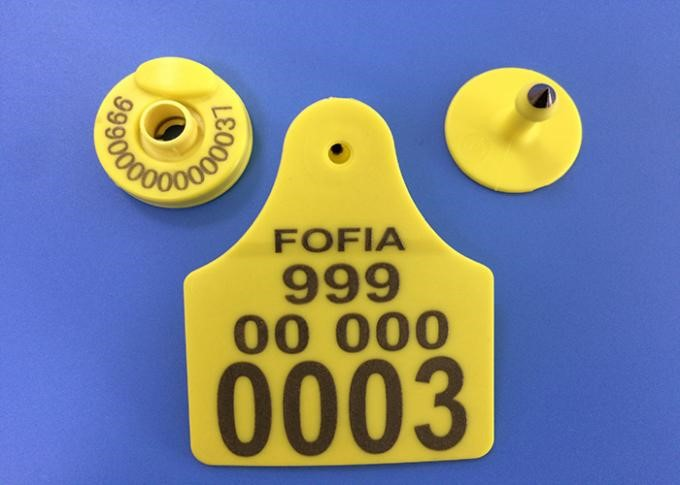
\includegraphics[scale = 0.4]{img/Modelo_de_etiqueta.jpg}
    \caption{Modelo de etiqueta.}
    \label{fig:modelo_etiqueta}
\end{figure}

{
Levando-se esses problemas em consideração, os Microcontroladores escolhidos para a realização dos estudos foram os referentes à família ESP e a família ATtiny, sendo seus principais polos o ESP8266, o ESP32 e o ATtiny13A-PU. Todos foram escolhidos por apresentarem alto desempenho em eficiência energética. Ademais, esses Microcontroladores apresentam a portabilidade de modelos de comunicação distintos, de modo que o ESP8266 possa utilizar o Wi-Fi, o ESP32 possa utilizar o BLE - Bluetooth Low Energy, e, por fim, o ATtiny13 possui compatibilidade com módulos de rádio frequência, como o NRF24l01.
}

{
Com tais Microcontroladores, pode-se contornar o problema de custo e autonomia, visto que se apresentam de fácil acesso e apresentam tecnologias já inclusas de baixo consumo. Além disso, apresentam boa compatibilidade com o tamanho total do projeto, facilitando a instalação na etiqueta.
}

{
Após a escolha dos referidos Microcontroladores, foram realizadas inúmeras análises de diversos modelos de baterias, com a finalidade de se obter o modelo que melhor atende às necessidades de tamanho, custo e capacidade energética, para acréscimo da autonomia. 
}

{
Mais especificamente, nesse projeto será montado um protótipo operacional de um dos nós da rede de integração de monitoramento do gado, utilizando um dos dois chips ESP, com o intuito de chegar a possíveis soluções para o projeto. Nas Figuras \ref{fig:prototipo_tamanho_esp32} e \ref{fig:prototipo_tamanho_esp8266}, apresentam-se as versões que servirão como base para os futuros protótipos, levando em consideração os modelos de bateria da mesma proporção, além dos pequenos componentes externos necessários para o funcionamento do circuito.
}

\begin{figure}[htp]
    \centering
    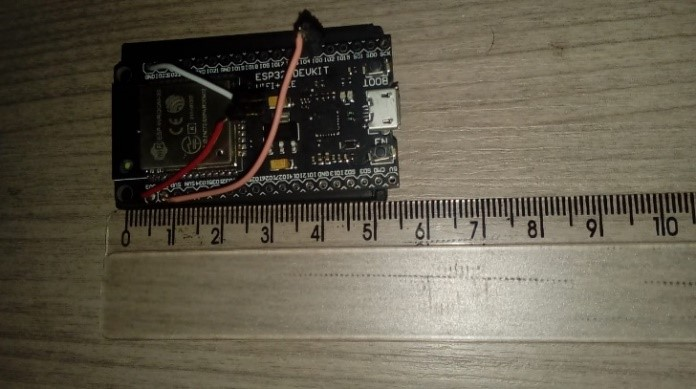
\includegraphics[scale = 0.9]{img/prototipo_ESP32_tamanho.jpg}
    \caption{Modelo de protótipo utilizando o ESP32}
    \label{fig:prototipo_tamanho_esp32}
\end{figure}

\begin{figure}[htp]
    \centering
    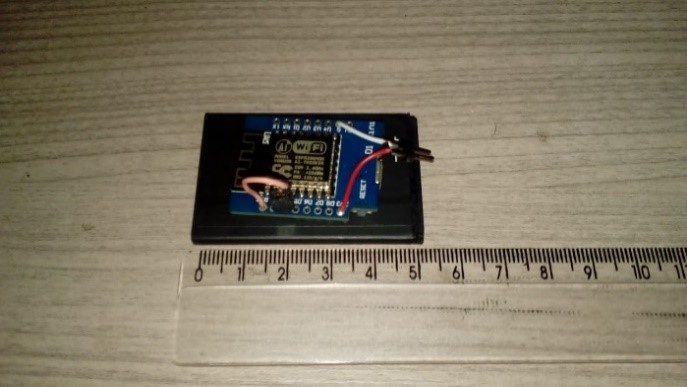
\includegraphics[scale = 0.9]{img/prototipo_ESP8266_tamanho.jpg}
    \caption{Modelo de protótipo utilizando o ESP8266}
    \label{fig:prototipo_tamanho_esp8266}
\end{figure}




\newpage
\section{Objetivos}
\label{sc:objetivos_}


{
Para apresentar uma nova forma de solução dos problemas enfrentados pelos fazendeiros, o objetivo é integrar múltiplas tecnologias, se apropriando do uso do IoT em conjunto com outros sistemas, tais como RSSI, Wi-Fi, Bluetooth Low Energy, criando um conjunto que possibilite ao fazendeiro gerenciar e localizar seu gado.
}

{
Esse sistema seria composto por antenas fixas espalhadas na área a ser monitorada e pela placa de transmissão acoplada na etiqueta de cada animal. No momento em que a placa acoplada transmite sinal para as antenas, o sinal seria processado e então serial calculada a sua localização aproximada por meio da trilateração, e esses dados ficariam dispostos ao agricultor.
}

{
A figura \ref{fig:modelo_simplificado_projeto} esboça de forma simplificada o sistema de transmissão de dados entre uma vaca com a placa desenvolvida acoplada em sua etiqueta de identificação entre duas antenas fixas. A partir dos cálculos realizados o fazendeiro poderá saber a localização aproximada da vaca em sua fazenda.
}

\begin{figure}[htp]
    \centering
    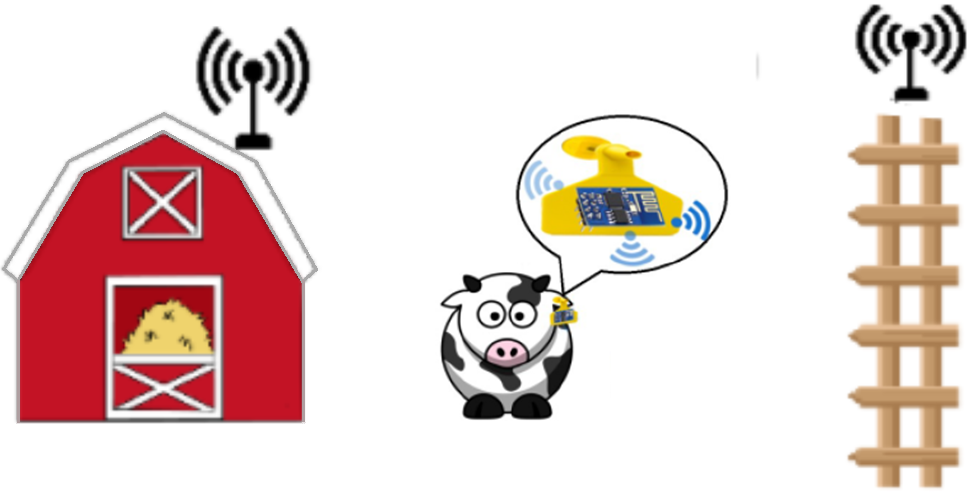
\includegraphics[scale = 0.5]{img/Resumo_projeto.png}
    \caption{Modelo simplificado projeto}
    \label{fig:modelo_simplificado_projeto}
\end{figure}



\newpage
\section{Material e Métodos}
\label{sc:metodologia_}



{
Inicialmente, foi realizada uma pesquisa dos diversos modelos e tipos de bateria para análise, com a finalidade de se optar por aquela que tenha maior eficiência nos critérios já mencionados (tamanho, custo e carga energética). Após a aferição de mais de 200 modelos diferentes, foram realizados vários filtros para a seleção destes, resultando na Tabela \ref{tabela:tabela_modelos_bateria_label} que possui vinte e oito modelos.
}


\label{sc:tabela_modelos_bateria}

\begin{table}[htp]
\caption{Tabela modelos de baterias}
\vspace{0.5cm}
\label{tabela:tabela_modelos_bateria_label}
\scalefont{0.6}
\begin{tabular}{|c|c|c|c|c|c|c|c|c|c|c|c|c|}
\hline
\multicolumn{1}{|c|}{\multirow{2}{*}{nº}} & \multicolumn{1}{c|}{\multirow{2}{*}{Marca}} & \multicolumn{1}{c|}{\multirow{2}{*}{Modelo}} & \multicolumn{1}{c|}{\multirow{2}{*}{Química}} & \multicolumn{3}{c|}{Dimensões(mm)} & \multicolumn{1}{c|}{\multirow{2}{*}{Tamanho}} & \multicolumn{1}{c|}{\multirow{2}{*}{Preço}} & \multicolumn{1}{c|}{\multirow{2}{*}{Tensão}} & \multicolumn{1}{c|}{\multirow{2}{*}{mAh}} & \multicolumn{1}{c|}{\multirow{2}{*}{Wh}} & \multicolumn{1}{c|}{\multirow{2}{*}{Custo/wh}} \\ \cline{5-7}
\multicolumn{1}{|c|}{}                           & \multicolumn{1}{c|}{}                       & \multicolumn{1}{c|}{}                        & \multicolumn{1}{c|}{}                                & C          & L         & A         & \multicolumn{1}{c|}{}                                   & \multicolumn{1}{c|}{}                       & \multicolumn{1}{c|}{}                                    & \multicolumn{1}{c|}{}                     & \multicolumn{1}{c|}{}                    & \multicolumn{1}{c|}{}                          \\[2pt] \hline
01                                               & Rontek                                      & RT300AAAB4                                   & Ni-cd                                                & 11         & 44        & 11        & Aaa                                                     & R\$4,98                                     & 1,20                                                     & 300,00                                    & 360,00                                   & 0,009722                                       \\[2pt] \hline 
02                                               & Energy Power                                & AA Ni-mh                                     & Ni-mh                                                & 14,5       & 50,5      & 14,5      & Aa                                                      & R\$8,90                                     & 1,20                                                     & 800,00                                    & 960,00                                   & 0,009271                                       \\[2pt] \hline
03                                               & Energy Power                                & AA Ni-cd                                     & Ni-cd                                                & 14,5       & 50,5      & 14,5      & Aa                                                      & R\$9,50                                     & 1,20                                                     & 1000,00                                   & 1.200,00                                 & 0,007917                                       \\[2pt] \hline
04                                               & Rontek                                      & AA Ni-mh                                     & Ni-mh                                                & 14,5       & 50,5      & 14,5      & Aa                                                      & R\$7,50                                     & 1,20                                                     & 2100,00                                   & 2.520,00                                 & 0,002976                                       \\[2pt] \hline
05                                               & Mox                                         & Aaa                                          & Ni-mh                                                & 14,5       & 50,5      & 14,5      & Aa                                                      & R\$3,80                                     & 1,20                                                     & 2700,00                                   & 3.240,00                                 & 0,001172                                       \\[2pt] \hline
06                                               & Knup                                        & KP-BT9V                                      & Ni-mh                                                & 47         & 20        & 15        & Bat P                                                   & R\$12,00                                    & 9,00                                                     & 450,00                                    & 4.050,00                                 & 0,002963                                       \\[2pt] \hline
07                                               & FLEX                                        & FX-45B1                                      & Ni-mh                                                & 47         & 20        & 15        & Bat P                                                   & R\$28,00                                    & 9,00                                                     & 450,00                                    & 4.050,00                                 & 0,008642                                       \\[2pt] \hline
08                                               & FullyMax                                    & -                                            & LIPO                                                 & 9,5        & 26        & 45        & Lipo M                                                  & R\$15,20                                    & 3,70                                                     & 650,00                                    & 2.405,00                                 & 0,006320                                       \\[2pt] \hline
09                                               & Mox                                         & MO-086B                                      & Ni-cd                                                & 31,5       & 44        & 10,5      & Aaa                                                     & R\$19,00                                    & 3,60                                                     & 700,00                                    & 2.520,00                                 & 0,001428                                       \\[2pt] \hline
10                                               & Rontek                                      & 6RT1800SC-CX                                 & Ni-cd                                                & 131        & 51        & 23        & Bat. G                                                  & R\$54,04                                    & 7,20                                                     & 1800,00                                   & 12.960,00                                & 0,004169                                       \\[2pt] \hline
11                                               & Rontek                                      & 6RT3000SC-CX                                 & Ni-mh                                                & 131        & 51        & 23        & Bat. G                                                  & R\$100,14                                   & 7,20                                                     & 3000,00                                   & 21.600,00                                & XXXX                                           \\[2pt] \hline
12                                               & Rontek                                      & 6LR61                                        & Ni-mh                                                & 48         & 26        & 16        & Bat. P                                                  & R\$18,50                                    & 8,40                                                     & 350,00                                    & 2.940,00                                 & XXXX                                           \\[2pt] \hline
13                                               & Rontek                                      & -                                            & Ni-mh                                                & 2          & 16        & 16        & P. Botão                                                & R\$5,15                                     & 3,60                                                     & 80,00                                     & 288,00                                   & XXXX                                           \\[2pt] \hline
14                                               & Rontek                                      & -                                            & Ni-mh                                                & 42         & 14        & 47        & 4 * Aaa                                                 & R\$9,86                                     & 3,60                                                     & 1300,00                                   & 4.680,00                                 & XXXX                                           \\[2pt] \hline
15                                               & Rontek                                      & -                                            & Ni-cd                                                & 17         & 51        & 57        & 3 * aa                                                  & R\$36,85                                    & 7,20                                                     & 600                                       & 4.320,00                                 & XXXX                                           \\[2pt] \hline
16                                               & FullyMax                                    & -                                            & LIPO                                                 & 7          & 20        & 36        & Lipo P                                                  & R\$14,40                                    & 3,70                                                     & 350,00                                    & 1.295,00                                 & 0,011119                                       \\[2pt] \hline
17                                               & minamoto                                    & LFP803048                                    & LiFePO4                                              & 8          & 30        & 50        & Lipo M                                                  & Orçamento                                   & 3,20                                                     & 800                                       & 2.560,00                                 & XXXX                                           \\[2pt] \hline
18                                               & minamoto                                    & LFP603450                                    & LiFePO4                                              & 6          & 34        & 50        & Lipo M                                                  & Orçamento                                   & 3,20                                                     & 700                                       & 2.240,00                                 & XXXX                                           \\[2pt] \hline
19                                               & minamoto                                    & LFP101945HP                                  & LiFePO4                                              & 10         & 19        & 45        & Lipo M                                                  & Orçamento                                   & 3,20                                                     & 440                                       & 1.408,00                                 & XXXX                                           \\[2pt] \hline
20                                               & minamoto                                    & LFP803048HP                                  & LiFePO4                                              & 8          & 30        & 48        & Lipo M                                                  & Orçamento                                   & 3,20                                                     & 800                                       & 2.560,00                                 & XXXX                                           \\[2pt] \hline
21                                               & minamoto                                    & LFR26650E                                    & LiFePO4                                              & 26         & 65        & 26        & D+                                                      & Orçamento                                   & 3,20                                                     & 3300                                      & 10.560,00                                & XXXX                                           \\[2pt] \hline
22                                               & minamoto                                    & LFR18650E                                    & LiFePO4                                              & 18,2       & 64,5      & 18,2      & D+                                                      & Orçamento                                   & 3,20                                                     & 1500                                      & 4.800,00                                 & XXXX                                           \\[2pt] \hline
23                                               & minamoto                                    & LFR18490E                                    & LiFePO4                                              & 18,2       & 48,5      & 18,2      & Aa                                                      & Orçamento                                   & 3,20                                                     & 1000                                      & 3.200,00                                 & XXXX                                           \\[2pt] \hline
24                                               & minamoto                                    & LFR14500E                                    & LiFePO4                                              & 14,1       & 48,5      & 14,1      & Aa                                                      & Orçamento                                   & 3,20                                                     & 500                                       & 1.600,00                                 & XXXX                                           \\[2pt] \hline
25                                               & minamoto                                    & LFR18650P                                    & LiFePO4                                              & 18,2       & 64,5      & 18,2      & D+                                                      & Orçamento                                   & 3,20                                                     & 1100                                      & 3.520,00                                 & XXXX                                           \\[2pt] \hline
26                                               & minamoto                                    & LFR26650P                                    & LiFePO4                                              & 26         & 65        & 26        & D+                                                      & Orçamento                                   & 3,20                                                     & 2300                                      & 7.360,00                                 & XXXX                                           \\[2pt] \hline
27                                               & minamoto                                    & LP104884                                     & LIPO                                                 & 10         & 48        & 84        & -                                                       & Orçamento                                   & 3,7                                                      & 5000                                      & 18.500,00                                & XXXX                                           \\[2pt] \hline
28                                               & FullyMax                                    & -                                            & LIPO                                                 & 10         & 26        & 45        & Lipo M                                                  & 27,20                                       & 3,7                                                      & 800                                       & 2.960,00                                 & 0,00125                                        \\[2pt] \hline
\end{tabular}
\end{table}



{
Logo após a separação desses vinte e oito modelos, foram realizadas novas pesquisas para delimitar possíveis características que filtrassem novamente os mesmos. Foram consultados os vários Datasheets\footnote{Datasheet é um arquivo digital a qual contém diversas informações técnicas do fabricante sobre um dado componente eletrônico. Sempre as informações mais confiáveis são fornecidas por esses arquivos.} referentes aos modelos de ESP e dos modos de funcionamento, chegando a especificamente cinco modelos que se apresentam como possíveis escolhas finais. Essas baterias serão adquiridas para a realização de experimentos práticos, para assim se chegar a uma conclusão definitiva.
}

{
De modo concomitante, para se chegar a um valor confiável do melhor modelo de bateria, foram realizados diversos testes experimentais, todavia, para efetuar tais testes foi feita uma placa shield, figura \ref{fig:placa_de_testes_01}, para a realização desses experimentos. Foi projetado um circuito, cujo esquemático feito no software Proteus (ver figura \ref{fig:esquematico_placa_de_testes_01}). Este, possui 8 leds que estão ligados em current source com 8 pinos digitais da placa WeMos, que serão controlados por um código fonte anteriormente programado. A placa foi projetada para drenar uma corrente fixa em cada digital I/O do ESP, para assim, aferir o consumo de corrente do chip.
}

\begin{figure}[H]
    \centering
    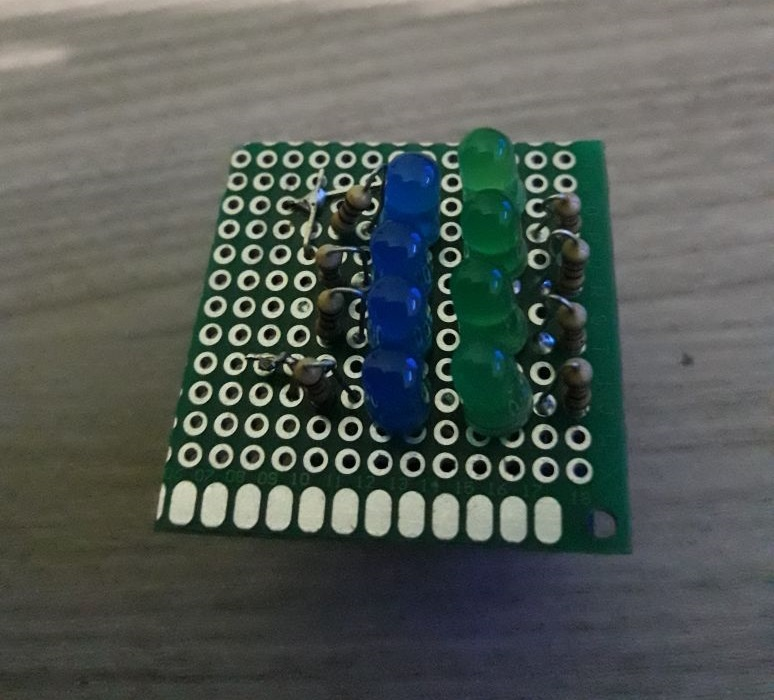
\includegraphics[scale = 0.3]{img/placa_de_testes_01.jpeg}
    \caption{Placa desenvolvida para aferição de consumo do ESP8266}
    \label{fig:placa_de_testes_01}
\end{figure}

\begin{figure}[htp]
    \centering
    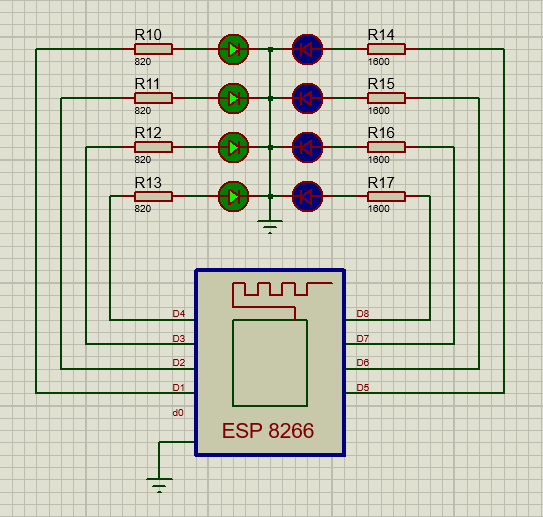
\includegraphics[scale = 0.5]{img/shield_01.png}
    \caption{Esquemático desenvolvido no proteus - Shield 1}
    \label{fig:esquematico_placa_de_testes_01}
\end{figure}

{
Após os primeiros testes de consumo do ESP, foram desenvolvidos diferentes códigos para que se possa aferir o consumo de energia por cada chip em cada modo de operação, modo de transmissão de dados e em cada modo de ‘Sleep\footnote{Sleep é o nome técnico dado ao período em que o processador não realiza grandes funções, como contas aritméticas ou transmissão de dados. Estes períodos de Sleep são utilizados basicamente para se poupar energia, visto que quando o processador entra neste modo, ele não realiza nenhuma operação que demande grande consumo de energia.}’. Cada um desses códigos foi desenvolvido utilizando o Arduino, software IDE, sendo que cada um foi programado utilizando a linguagem C++. Após esta etapa, os códigos foram armazenados, junto aos demais arquivos do projeto, na plataforma Git Hub, com o nome “W8jonas”.
}

{
Ao final da etapa de programação e de aferição do consumo de corrente pela shield 1. Foi feita uma segunda shield, (ver figura \ref{fig:placa_de_testes_02}), capaz d alterar entre os diferentes modos de funcionamento por meio de um botão. O códigoe fonte inserido na placa ESP permite a troca de funções exercidas pelo ESP, desse modo, a cada pressionar do botão, uma nova forma de funcionamento é estabelecida. 
}

\begin{figure}[htp]
    \centering
    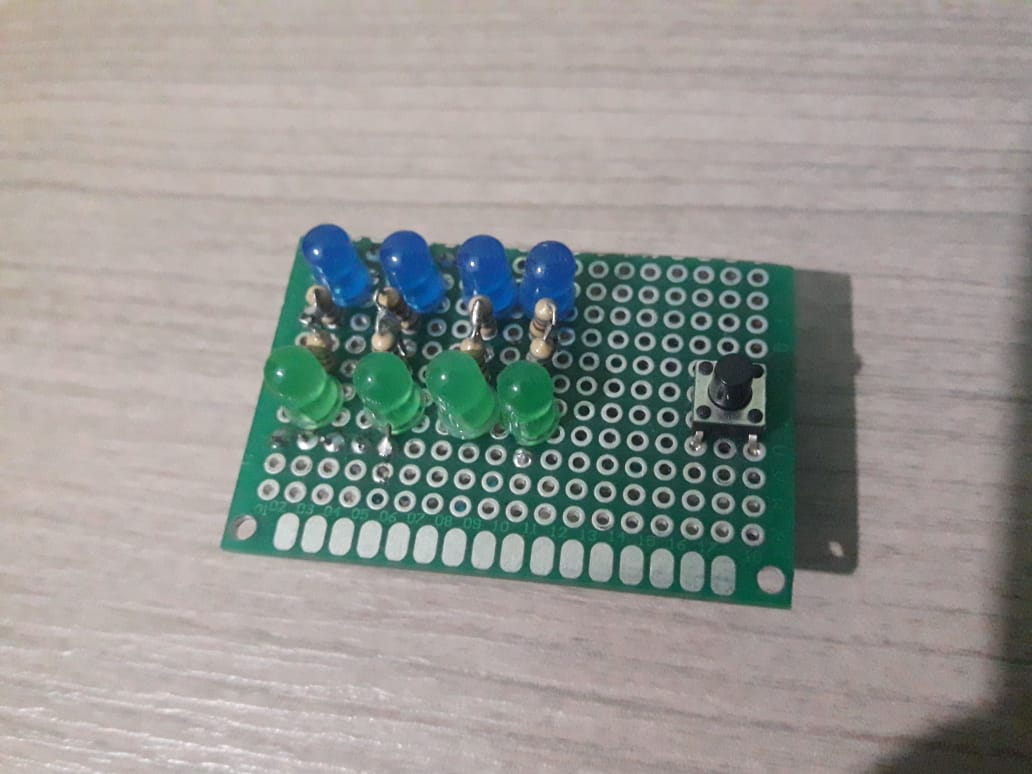
\includegraphics[scale = 0.3]{img/placa_de_testes_02.jpeg}
    \caption{Placa desenvolvida para controlar as funções do ESP}
    \label{fig:placa_de_testes_02}
\end{figure}

{
O código tem como objetivo estabelecer 6 funções diferentes para o Arduino executar cada uma delas de modo separado. Esse programa apresenta dois principais núcleos de funcionamento, a leitura do pressionar do botão, cuja a lógica é compreendida entre as chaves do comando void setup(){ }, e a parte da alteração das funções, em cada função declarada demonstra um modo de funcionamento diferente.
\newline
O código fonte em específico encontra-se na íntegra abaixo:
}

{
\begin{lstlisting}

//  Internet das Vacas código 3
//  Autor: Jonas Henriquee Nascimento
//  PIBIC-Junior
//
//  Data de início: 04/06/2018
//  Data da ultima atualização: 19/06/2018
//  Data de término: 08/06/2018
//  
//  O código tem como objetivo estabelecer 6 funções diferentes para o arduino
//  executar cada uma delas de moto paralelo. Essas funções são escolhidas através 
//  de um botão que toda que apertado faz com que o código execute a função seguinte
//  A primeira função, que é executada junto ao ESP quando é ligado deixa todos os
//  LEDs desligados e o ESP em modo de standby. A segunda função, liga somente um
//  dos LEDs. A terceira, por sua vez, liga todos os 8 LEDs. A próxima função 
//  executa uma série de operações aritméticas, com todos os LEDs desligados. Já a 
//  função 5 executa as mesmas operações aritméticas, mas com 1 dos LEDs ligados. 
//  De tal forma é feito na 6 função, no qual são executadas as operações matemáticas,
//  mas com todos os LEDs ligados.

//  Este código está disponível sempre no endereço abaixo, para livre aperfeiçoamento. 
//  Todavia, pede-se por educação, que ao compartilharem o código, mantenham os autores
//  originais, tão bem quanto o nome da instituição.
//  https://github.com/W8jonas/Internet-das-Vacas/blob/master/programacao/codigo_modos_de_operacao/codigo_modos_de_operacao.ino




#define Output_1 D8
#define Output_2 D7
#define Output_3 D6
#define Output_4 D5
#define Output_5 D4
#define Output_6 D3
#define Output_7 D2
#define Output_8 D1
#define entrada_botao D0

void funcao__();
void funcao_0();
void funcao_1();
void funcao_2();
void funcao_3();
void funcao_4();

int operacao = 0;
boolean leitura = true;

void setup() {
   pinMode (Output_1, OUTPUT);
   pinMode (Output_2, OUTPUT);
   pinMode (Output_3, OUTPUT);
   pinMode (Output_4, OUTPUT);
   pinMode (Output_5, OUTPUT);
   pinMode (Output_6, OUTPUT);
   pinMode (Output_7, OUTPUT);
   pinMode (Output_8, OUTPUT);
   pinMode (entrada_botao, INPUT);
   Serial.begin(115200);
}

void loop() {
  leitura = digitalRead(entrada_botao);
  Serial.println(leitura);
  if (leitura == LOW ){
     operacao++;
     delay(500);
  }

  funcao_2(); 

}

void funcao__ (){
   Serial.println("funcao 00 ");
   digitalWrite(Output_1, LOW);
   digitalWrite(Output_2, LOW);
   digitalWrite(Output_3, LOW);
   digitalWrite(Output_4, LOW);
   digitalWrite(Output_5, LOW);
   digitalWrite(Output_6, LOW);
   digitalWrite(Output_7, LOW);
   digitalWrite(Output_8, LOW);
}

void funcao_0() {
   Serial.println("funcao 0 ");
   digitalWrite(Output_1, HIGH);
}

void funcao_1() {
   Serial.println("funcao 1 ");
   digitalWrite(Output_1, HIGH);
   digitalWrite(Output_2, HIGH);
   digitalWrite(Output_3, HIGH);
   digitalWrite(Output_4, HIGH);
   digitalWrite(Output_5, HIGH);
   digitalWrite(Output_6, HIGH);
   digitalWrite(Output_7, HIGH);
   digitalWrite(Output_8, HIGH);
}

void funcao_2() {
   Serial.println("funcao 2 ");
   digitalWrite(Output_1, LOW);
   digitalWrite(Output_2, LOW);
   digitalWrite(Output_3, LOW);
   digitalWrite(Output_4, LOW);
   digitalWrite(Output_5, LOW);
   digitalWrite(Output_6, LOW);
   digitalWrite(Output_7, LOW);
   digitalWrite(Output_8, LOW);
   int cont = 1;
   float resp = 1;
   float resp2 = 1;
   for(int AA = 0; AA < 500; AA++){
      resp = 3 + sin(resp)/cos(resp*resp/2) * sqrt(sqrt(resp*resp));
      resp = resp * 0.5;
      resp2 = sqrt(AA);
      yield();
  }
}

void funcao_3() {
   Serial.println("funcao 3 ");
   digitalWrite(Output_1, HIGH);
   int cont = 1;
   float resp = 1;
   float resp2 = 1;
   for(int AA = 0; AA < 500; AA++){
      resp = 3 + sin(resp)/cos(resp*resp/2) * sqrt(sqrt(resp*resp));
      resp = resp * 0.5;
      resp2 = sqrt(AA);
      yield();
  }
}

void funcao_4() {
   Serial.println("funcao 4 ");
   digitalWrite(Output_1, HIGH);
   digitalWrite(Output_2, HIGH);
   digitalWrite(Output_3, HIGH);
   digitalWrite(Output_4, HIGH);
   digitalWrite(Output_5, HIGH);
   digitalWrite(Output_6, HIGH);
   digitalWrite(Output_7, HIGH);
   digitalWrite(Output_8, HIGH);
   int cont = 1;
   float resp = 1;
   float resp2 = 1;
   for(int AA = 0; AA < 500; AA++){
      resp = 3 + sin(resp)/cos(resp*resp/2) * sqrt(sqrt(resp*resp));
      resp = resp * 0.5;
      resp2 = sqrt(AA);
      yield();
  }
}

\end{lstlisting}
}

{
Além deste código, foram desenvolvidos outros códigos para o funcionamento de outros modos tratamento de transmissão de sinais, incluindo, também, diferentes formas de economia de energia. Novamente, utilizou-se do pressionar do botão para a alteração entre as funções relativas a cada estado de funcionamento do ESP. Todos os demais códigos feitos encontram-se nos Apêndices deste documento.
}

{
Nesse momento, foram realizadas medidas de consumo de corrente, para isso foram utilizados três multímetros de marcas e modelos diferentes, sendo suas aferições relatadas em maior valor lido e menor valor lido. A tensão foi medida em um resistor shunt de 1 Ω em série com o protótipo de teste de consumo. Após a coleta das seis medidas, foi calculada a média aritmética para se chegar ao resultado final de consumo. A tabela \ref{tabela:tabela_resumo_de_consumo_ESP8266}  apresenta, sucintamente, os valores obtidos, todos os valores medidos, incluindo todas as características dos modos de funcionamento estão dispostos na tabela apresentada no apêndice A.
}


\begin{table}[htp]
\caption{Tabela resumo de consumo ESP8266}
\vspace{0.5cm}
\label{tabela:tabela_resumo_de_consumo_ESP8266}
\begin{tabular}{|l|l|l|}
\hline
Modo de operação                                                     & Configurações do modo      & Consumo médio (mA) \\ \hline
Standby                                                              & VCC = 5v                   & 75,333             \\ \hline
1 Led ligado                                                         & VCC = 5v                   & 75,583             \\ \hline
\begin{tabular}[c]{@{}l@{}}Todos os Leds\\   ligados\end{tabular}    & VCC = 5v                   & 79,3               \\ \hline
100\% uso do CPU                                                     & VCC = 5v                   & 76,9               \\ \hline
\begin{tabular}[c]{@{}l@{}}1 Led ligado + 100\%\\   CPU\end{tabular} & VCC = 5v                   & 77,783             \\ \hline
Todos os Leds + 100\% CPU                                            & VCC = 5v                   & 80,333             \\ \hline
ESP server e cliente ligado                                          & VCC = 5v                   & 75,366             \\ \hline
ESP only client                                                      & VCC = 5v                   & 71,983             \\ \hline
Modem Sleep                                                          & VCC = 5v                   & 71,933             \\ \hline
Light Sleep – CPU ativa                                              & VCC = 5v                   & 16,4               \\ \hline
Light Sleep – CPU desativada                                         & VCC = 5v                   & 2,23               \\ \hline
\multirow{2}{*}{Deep Sleep}                                          & VCC = 5v                   & 0,133              \\ \cline{2-3} 
                                                                     & VCC = 3.3v                 & 0,011              \\ \hline
\multirow{2}{*}{Transmit 802.11b}                                    & VCC = 5v e POUT = +20.5dBm & 75,233             \\ \cline{2-3} 
                                                                     & VCC = 5v e POUT = +14dBm   & 74,866             \\ \hline
\multirow{2}{*}{Transmit 802.11g}                                    & VCC = 5v e POUT = +20.5dBm & 74,050             \\ \cline{2-3} 
                                                                     & VCC = 5v e POUT = +14dBm   & 71,116             \\ \hline
\multirow{2}{*}{Transmit 802.11n}                                    & VCC = 5v e POUT = +20.5dBm & 71,433             \\ \cline{2-3} 
                                                                     & VCC = 5v e POUT = +14dBm   & 71,250             \\ \hline
\end{tabular}
\end{table}

{
Após os valores aferidos, foi feita uma análise de autonomia em relação ao modelo de bateria e aos modos de funcionamento do ESP8266. O padrão de comportamento do chip se apresenta de maneira análoga em todos os casos de análise, pois o funcionamento se baseia em um tempo com o processador ligado, um período com o transmissor de sinais ligado, e um período de Sleep. Esse padrão foi definido dessa forma porque apresenta melhor rendimento.
}

{

}

{
Inicialmente, após a coleta dos dados de consumo, foram criadas equações matemáticas que estimam, de modo aproximado, o gasto energético da placa em diferentes modos de funcionamento com a carga energética das baterias selecionadas, calculando, dessa forma, os valores de autonomia do protótipo. O Gráfico \ref{grafico:grafico_consumo_linear} mostra a relação dos modos de operação selecionados e sua autonomia, tomando como exemplo uma bateria de carga energética igual a 650 mAh. 
}

\begin{figure}[htp]
    \centering
    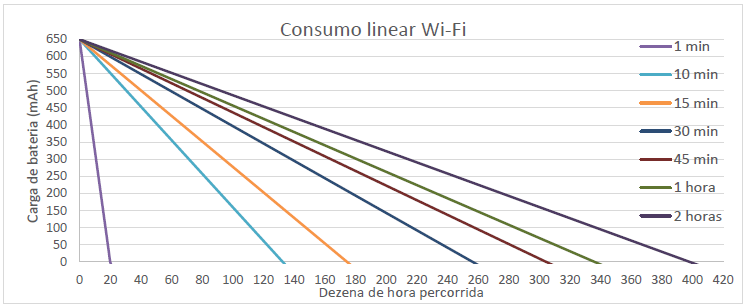
\includegraphics[scale = 0.8]{img/grafico_consumo_linear_prototipo.png}
    \caption{Gráfico consumo linear protótipo 1}
    \label{grafico:grafico_consumo_linear}
\end{figure}

{
Cada modo de operação do Chip possui vantagens e desvantagens, que serão aprimoradas posteriormente junto à codificação final do projeto. Vale salientar que a principal diferença entre os modos está na velocidade dos rastreamentos realizados, sendo que quanto menor o tempo de repetição, mais precisa será a localização. Caso o tempo fosse zero, o monitoramento seria considerado em tempo real, o que se torna possível, mas não viável, pelo alto custo de se manter este sistema funcionando por um longo período.
}

{
A partir das análises preliminares do gráfico, é possível destacar a diferença entre a melhor curva e a pior curva de consumo, destacando, dessa forma, como a pouca diferença entre algumas variáveis altera o resultado final. De certo modo, é impossível que se tenha uma precisão de 100\% no valor de autonomia, isso se deve a dois principais motivos. 
}

{
O primeiro fator se deve a curva de descarga da bateria, a qual não é inteiramente linear, apresentando em seu início e fim curvas exponenciais, dificultando, dessa maneira, os cálculos precisos com relação a descarga da bateria. Essas curvas estão diretamente ligadas aos tipos químicos de cada bateria e os diferentes modelos produzidos por cada empresa da área.
}

{
O segundo fator direciona-se ao fato que os próprios chips possuem variantes internos, estes que por sua vez variam naturalmente, além de serem susceptíveis a variações externas como temperatura. Logo, com variações externas, soma-se as variações resultantes do código fonte executado pelo ESP8266, de suas contas e de suas variações com o decorrer do tempo. Ademais, soma-se as variações de corrente consumida pelo chip em consequência das variações de tensão fornecida pela bateria, visto que esta, ao passar do tempo, tende a diminuir.
}

{
Após os primeiros testes experimentais, foi projetado e montado um circuito capaz de analisar em tempo real os valores de tensão da bateria em decorrer do funcionamento dos chips ESPs em diferentes modelos de bateria. O experimento foi realizado para que se possa aferir divergências entre os valores obtidos teoricamente e os obtidos no funcionamento dos circuitos.
}

{
O funcionamento deste circuito, rotulado de “Circuito datalogger de tensão”, tem como função ler, a cada minuto, o valor de tensão de cada uma das baterias dispostas no circuito que alimentam determinado ESP e armazenar os valores em um arquivo do tipo ‘.svc’ para a análise em algum programa.
}

{
Inicialmente foram gravados os mesmos códigos com suas adaptações tanto para o ESP32 quando para o ESP8266, no qual eram responsáveis por operar o protótipo de modo a seguir o padrão de consumo/funcionamento referente a tabela \ref{tabela:tabela_modos_de_operacao}.
}

\begin{table}[htp]
\caption{Tabela modo de funcionamento}
\vspace{0.5cm}
\label{tabela:tabela_modos_de_operacao}
\scalefont{0.6}
\begin{tabular}{lllllllllll}
\cline{1-4}
\multicolumn{2}{|l|}{Especificações:}                                                                                    & \multicolumn{1}{c|}{Valor}                                    & \multicolumn{1}{c|}{Unidade}                        &                                                     &                                                      &                                                                        &                                                                      &                                                                        &                                                                     &                                                                     \\ \cline{1-4}
\multicolumn{1}{|l|}{}                                            & \multicolumn{1}{l|}{bateria}                         & \multicolumn{1}{l|}{750}                                      & \multicolumn{1}{l|}{mAh}                            &                                                     &                                                      &                                                                        &                                                                      &                                                                        &                                                                     &                                                                     \\ \cline{1-4}
\multicolumn{1}{|l|}{}                                            & \multicolumn{1}{l|}{bateria}                         & \multicolumn{1}{l|}{2700000}                                  & \multicolumn{1}{l|}{mAsec}                          &                                                     &                                                      &                                                                        &                                                                      &                                                                        &                                                                     &                                                                     \\ \cline{1-4}
                                                                  &                                                      &                                                               &                                                     &                                                     &                                                      &                                                                        &                                                                      &                                                                        &                                                                     &                                                                     \\ \hline
\multicolumn{1}{|c|}{Teste}                                       & \multicolumn{1}{c|}{Running}                         & \multicolumn{1}{c|}{Operação}                                 & \multicolumn{1}{c|}{Consumo}                        & \multicolumn{1}{c|}{Tempo de}                       & \multicolumn{1}{c|}{Consumo}                         & \multicolumn{1}{c|}{Consumo}                                           & \multicolumn{1}{c|}{Consumo por}                                     & \multicolumn{1}{c|}{Número de}                                         & \multicolumn{2}{c|}{Duração total}                                                                                                        \\ \cline{10-11} 
\multicolumn{1}{|l|}{(nº)}                                        & \multicolumn{1}{l|}{}                                & \multicolumn{1}{l|}{}                                         & \multicolumn{1}{l|}{(mA)}                           & \multicolumn{1}{l|}{operação (s)}                   & \multicolumn{1}{l|}{(mAsec)}                         & \multicolumn{1}{l|}{por ciclo}                                         & \multicolumn{1}{l|}{hora (mAh)}                                      & \multicolumn{1}{l|}{ciclos possíveis}                                  & \multicolumn{1}{l|}{Em horas}                                       & \multicolumn{1}{l|}{Em dias}                                        \\ \hline
\rowcolor[HTML]{C0C0C0} 
\multicolumn{1}{|c|}{\cellcolor[HTML]{C0C0C0}}                    & \multicolumn{1}{l|}{\cellcolor[HTML]{C0C0C0}Valor X} & \multicolumn{1}{l|}{\cellcolor[HTML]{C0C0C0}Deep Sleep}       & \multicolumn{1}{l|}{\cellcolor[HTML]{C0C0C0}0,133}  & \multicolumn{1}{l|}{\cellcolor[HTML]{C0C0C0}100,00} & \multicolumn{1}{l|}{\cellcolor[HTML]{C0C0C0}13,30}   & \multicolumn{1}{l|}{\cellcolor[HTML]{C0C0C0}}                          & \multicolumn{1}{l|}{\cellcolor[HTML]{C0C0C0}}                        & \multicolumn{1}{l|}{\cellcolor[HTML]{C0C0C0}}                          & \multicolumn{1}{l|}{\cellcolor[HTML]{C0C0C0}}                       & \multicolumn{1}{l|}{\cellcolor[HTML]{C0C0C0}}                       \\ \cline{2-6}
\rowcolor[HTML]{C0C0C0} 
\multicolumn{1}{|c|}{\cellcolor[HTML]{C0C0C0}}                    & \multicolumn{1}{l|}{\cellcolor[HTML]{C0C0C0}Valor Y} & \multicolumn{1}{l|}{\cellcolor[HTML]{C0C0C0}100\% uso do CPU} & \multicolumn{1}{l|}{\cellcolor[HTML]{C0C0C0}76,900} & \multicolumn{1}{l|}{\cellcolor[HTML]{C0C0C0}20,00}  & \multicolumn{1}{l|}{\cellcolor[HTML]{C0C0C0}1538,00} & \multicolumn{1}{l|}{\cellcolor[HTML]{C0C0C0}}                          & \multicolumn{1}{l|}{\cellcolor[HTML]{C0C0C0}}                        & \multicolumn{1}{l|}{\cellcolor[HTML]{C0C0C0}}                          & \multicolumn{1}{l|}{\cellcolor[HTML]{C0C0C0}}                       & \multicolumn{1}{l|}{\cellcolor[HTML]{C0C0C0}}                       \\ \cline{2-6}
\rowcolor[HTML]{C0C0C0} 
\multicolumn{1}{|c|}{\multirow{-3}{*}{\cellcolor[HTML]{C0C0C0}1}} & \multicolumn{1}{l|}{\cellcolor[HTML]{C0C0C0}Valor W} & \multicolumn{1}{l|}{\cellcolor[HTML]{C0C0C0}Transmit 802.11n} & \multicolumn{1}{l|}{\cellcolor[HTML]{C0C0C0}71,433} & \multicolumn{1}{l|}{\cellcolor[HTML]{C0C0C0}5,00}   & \multicolumn{1}{l|}{\cellcolor[HTML]{C0C0C0}357,16}  & \multicolumn{1}{l|}{\multirow{-3}{*}{\cellcolor[HTML]{C0C0C0}1908,46}} & \multicolumn{1}{l|}{\multirow{-3}{*}{\cellcolor[HTML]{C0C0C0}15,26}} & \multicolumn{1}{l|}{\multirow{-3}{*}{\cellcolor[HTML]{C0C0C0}1414,74}} & \multicolumn{1}{l|}{\multirow{-3}{*}{\cellcolor[HTML]{C0C0C0}49,1}} & \multicolumn{1}{l|}{\multirow{-3}{*}{\cellcolor[HTML]{C0C0C0}2,05}} \\
\rowcolor[HTML]{C0C0C0} 
\multicolumn{1}{|l|}{\cellcolor[HTML]{C0C0C0}}                    & \multicolumn{1}{l|}{\cellcolor[HTML]{C0C0C0}}        & \multicolumn{1}{l|}{\cellcolor[HTML]{C0C0C0}POUT = + 20.5dBm} & \multicolumn{1}{l|}{\cellcolor[HTML]{C0C0C0}}       & \multicolumn{1}{l|}{\cellcolor[HTML]{C0C0C0}}       & \multicolumn{1}{l|}{\cellcolor[HTML]{C0C0C0}}        & \multicolumn{1}{l|}{\cellcolor[HTML]{C0C0C0}}                          & \multicolumn{1}{l|}{\cellcolor[HTML]{C0C0C0}}                        & \multicolumn{1}{l|}{\cellcolor[HTML]{C0C0C0}}                          & \multicolumn{1}{l|}{\cellcolor[HTML]{C0C0C0}}                       & \multicolumn{1}{l|}{\cellcolor[HTML]{C0C0C0}}                       \\ \hline
\multicolumn{1}{|c|}{}                                            & \multicolumn{1}{l|}{Valor X}                         & \multicolumn{1}{l|}{Deep Sleep}                               & \multicolumn{1}{l|}{0,133}                          & \multicolumn{1}{l|}{100,00}                         & \multicolumn{1}{l|}{13,30}                           & \multicolumn{1}{l|}{}                                                  & \multicolumn{1}{l|}{}                                                & \multicolumn{1}{l|}{}                                                  & \multicolumn{1}{l|}{}                                               & \multicolumn{1}{l|}{}                                               \\ \cline{2-6}
\multicolumn{1}{|c|}{}                                            & \multicolumn{1}{l|}{Valor Y}                         & \multicolumn{1}{l|}{100\% uso do CPU}                         & \multicolumn{1}{l|}{76,900}                         & \multicolumn{1}{l|}{200,00}                         & \multicolumn{1}{l|}{15380,00}                        & \multicolumn{1}{l|}{}                                                  & \multicolumn{1}{l|}{}                                                & \multicolumn{1}{l|}{}                                                  & \multicolumn{1}{l|}{}                                               & \multicolumn{1}{l|}{}                                               \\ \cline{2-6}
\multicolumn{1}{|c|}{\multirow{-3}{*}{2}}                         & \multicolumn{1}{l|}{Valor W}                         & \multicolumn{1}{l|}{Transmit 802.11n}                         & \multicolumn{1}{l|}{71,433}                         & \multicolumn{1}{l|}{200,00}                         & \multicolumn{1}{l|}{14286,60}                        & \multicolumn{1}{l|}{\multirow{-3}{*}{29679,90}}                        & \multicolumn{1}{l|}{\multirow{-3}{*}{59,36}}                         & \multicolumn{1}{l|}{\multirow{-3}{*}{90,97}}                           & \multicolumn{1}{l|}{\multirow{-3}{*}{12,6}}                         & \multicolumn{1}{l|}{\multirow{-3}{*}{0,53}}                         \\
\multicolumn{1}{|l|}{}                                            & \multicolumn{1}{l|}{}                                & \multicolumn{1}{l|}{POUT = + 20.5dBm}                         & \multicolumn{1}{l|}{}                               & \multicolumn{1}{l|}{}                               & \multicolumn{1}{l|}{}                                & \multicolumn{1}{l|}{}                                                  & \multicolumn{1}{l|}{}                                                & \multicolumn{1}{l|}{}                                                  & \multicolumn{1}{l|}{}                                               & \multicolumn{1}{l|}{}                                               \\ \hline
\end{tabular}
\end{table}


{
O circuito teve como centro o Arduino Mega, a qual serviu de ponte entre a leitura de tensão de cada bateria ligada à um diferente ESP e o armazenamento dessas leituras em um cartão de memória. Para a leitura e o registro serem feitos com sucesso e uma coerente exatidão, foram utilizados dois módulos ao Arduino Mega, o módulo ‘Cartão SD’ e o módulo ‘RTC – Real Time Clock’. Todo seu esquemático pode ser observado na figura \ref{fig:esquematico_datalogger_de_tensao}. Todavia, seu esquemático se apresenta em um nível alto de abstração, visto que os componentes foram representados por meros blocos gráficos, porém, assim, não interferindo na análise do circuito, a partir de seu esquemático.
}

\begin{figure}[H]
    \centering
    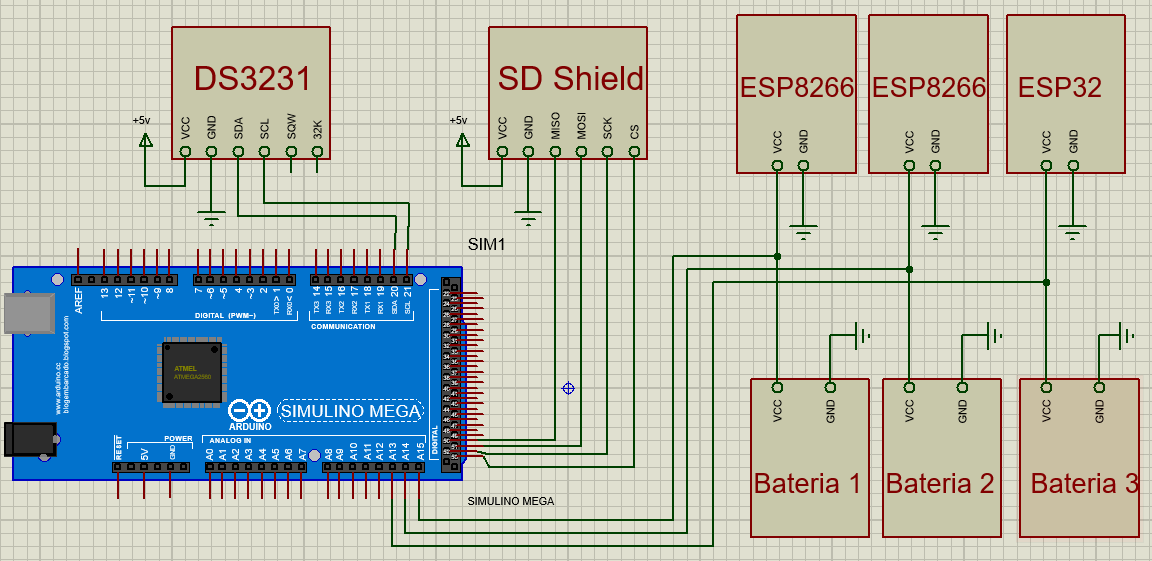
\includegraphics[scale = 0.55]{img/esquematico_datalogger_de_tensao.png}
    \caption{Esquemático do circuito Datalogger de tensão}
    \label{fig:esquematico_datalogger_de_tensao}
\end{figure}

{
Cada um dos módulos teve suas funções bem definidas. O ‘Cartão SD’ foi utilizado para armazenar todos os dados colhidos das leituras, contendo a data e hora da medida, que foram extraídos do RTC. As gravações foram feitas em um arquivo de nome “TENSOEX.SVC”, onde ‘X’ representa o número do teste. Como por exemplo, o teste número 3 teve nome igual a: “TENSOE3.SVC”. 
}

{
Dentro desse arquivo, foram armazenados os dados separados por um caractere indicador, nos primeiros testes, foi escolhido o caractere ‘, ’, porém, após algumas análises, o caractere escolhido foi substituído para ‘; ’. Isso foi feito para que, após o termino das gravações, o arquivo possa ser aberto utilizando algum software para tabulações, o mais conhecido, e que foi utilizado é o Microsoft Excel. A partir dele, é possível abrir esse arquivo e colocar cada valor lido separado em uma célula para posteriormente trabalhar com alguma aplicação no Excel, como a construção de gráficos comparativos. 
}

{
Os dados foram mantidos em uma hierarquização de ordem, em outras palavras, todos os dados foram sempre armazenados na mesma ordem, com a finalidade de se manter um padrão e facilitar a aplicabilidade em diversos programas de tabulação. A ordem escolhida para a escrita no cartão de memória foi: data, hora, valor do sensor 1, valor do sensor 2, erro 1, erro 2, ||; Dessa forma, os dados foram gravados como demonstrado na tabela \ref{tabela:tabela_dados_gravados}:
}


\begin{table}[htp]
\caption{Valores gravados no cartão para análise}
\vspace{0.5cm}
\label{tabela:tabela_dados_gravados}
\scalefont{0.8}
\centering
\begin{tabular}{
>{\columncolor[HTML]{EFEFEF}}l }
\hline
\multicolumn{1}{|c|}{\cellcolor[HTML]{EFEFEF}
11.09.2018; 16:56:00; 3.51; 3.57; 3; 2; ||;} \\ \hline
11.09.2018; 16:57:00; 3.51; 3.56; 3; 2; ||;  \\
11.09.2018; 16:58:00; 3.50; 3.55; 4; 2; ||;  \\
11.09.2018; 16:59:00; 3.50; 3.54; 4; 2; ||;  \\
11.09.2018; 17:00:00; 3.50; 3.53; 4; 2; ||;
\end{tabular}
\end{table}

{
Logo, transcrevendo as informações, temos os dados contidos na tabela \ref{tabela:tabela_dados_contidos_na_gravacao}:
}

\begin{table}[htp]
\caption{Dados contidos na gravação do cartão para análise}
\vspace{0.5cm}
\label{tabela:tabela_dados_contidos_na_gravacao}
\centering
\begin{tabular}{|
>{\columncolor[HTML]{EFEFEF}}l |}
Data: 11.09.2018                            \\
Horas: 16:56:00                             \\
Valor do sensor 1: 3.51                     \\
Valor do sensor 2: 3.57                     \\
Erro 1: 4                                   \\
Erro 2: 2                                   \\
|| : Caractere sinalizador de fim de linha.
\end{tabular}
\end{table}


{
A cada nova leitura de tensão nas baterias, é escrito uma nova linha, logo abaixo do anterior, com a exata mesma sintaxe. Todavia, com seus dados atualizados com os novos valores referentes a leitura. 
}

{
Todo o código fonte pode ser observado abaixo: \newline
}

\begin{lstlisting}

/*
 * Instituto Federal de Educação, Ciência e Tecnologia Minas Gerais
 * IFMG - Campus Avançado Conselheiro Lafaiete 
 * 
 * Internet das Vacas código monitoramento de tensão
 * Autor: Jonas Henrique Nascimento
 * PIBIC-Junior
 * 
 * Data de início.................: 06/09/2018
 * Data da ultima atualização.....: 23/09/2018
 * Data de atualização de versão..: 23/09/2018
 * Data de término................: 23/09/2018
 * 
 * 
 * 
 *  Este código está disponível sempre no endereço abaixo, para livre aperfeiçoamento. 
 *  Todavia, pede-se por educação, que ao compartilharem o código, mantenham os autores
 *  originais, tão bem quanto o nome da instituição.
 *  
 *  https://github.com/W8jonas/Internet-das-Vacas/blob/master/programacao/Monitoramento_de_tensao_2.1/Monitoramento_de_tensao_2.1.ino
 *  
*/


#include <DS3231.h>
#include <SPI.h>
#include <SD.h>
#define chip_select 4


int pino_sensor_de_tensao_ESP32 = A0;             // pino do arduino utilizado para medir a tensao da bateria ligada ao ESP32
float valor_do_sensor_de_tensao_ESP32 = 0;        // variavel de ponto flutuante que armazena o valor de tensao lido do ESP32
                                                  //
int pino_sensor_de_tensao_ESP8266 = A8;           // pino do arduino utilizado para medir a tensao da bateria ligada ao ESP8266
float valor_do_sensor_de_tensao_ESP8266 = 0;      // variavel de ponto flutuante que armazena o valor de tensao lido do ESP8266


int pino_sensor_controle_ESP32 = A1;              // Valor lido de tensao para converter em estado de HIGH ou LOW
float valor_do_sensor_de_controle_ESP32 = 0;      // Valor armazenado de tensao
                                                  //
int pino_sensor_controle_ESP8266 = A9;            // Valor lido de tensao para converter em estado de HIGH ou LOW
float valor_do_sensor_de_controle_ESP8266 = 0;    // Valor armazenado de tensao


unsigned int minuto_antigo = 0;
unsigned int minuto_atual = 0;
unsigned int marcador_tempo_1 = 0;
unsigned int marcador_tempo_2 = 0;

bool flag = false;
bool flag2 = false;
bool flag_controle_marcador_ON = false;
bool flag_controle_marcador_OFF = false;
bool flag_ligado = false;

String texto_marcador = "string marcador";
String dados = "string dados";
String condicao_ = "condicao";

unsigned char erro_marcador_1 = 0;
unsigned char erro_marcador_2 = 0;

void leitura();
void marcador(String marcador);
void gravar_dados_cartao();

DS3231  rtc(SDA, SCL);
Time  t;
File datalogger;

void setup() {
  
   Serial.begin(115200);
   rtc.begin();
   while (!Serial) {;}
   
   if (!SD.begin(chip_select)) {
     Serial.println("Erro ao ler cartao de memoria");
     return;
  }
  
}


void loop() {
   t = rtc.getTime();
   minuto_atual = t.min;
   
   if ( digitalRead(10) == HIGH) {
      condicao_ = "LIGADO";
      marcador(condicao_);
   } else {
      condicao_ = "DESLIGADO";
      marcador(condicao_);
   }
   
   if ( minuto_antigo != minuto_atual ){  
      minuto_antigo = minuto_atual;
      leitura();
      dados = texto_marcador + rtc.getDateStr() + ";" + rtc.getTimeStr() + ";" + valor_do_sensor_de_tensao_ESP8266 + ";" + valor_do_sensor_de_tensao_ESP8266 + ";" + erro_marcador_1 + ";" + erro_marcador_2 + ";*";
      gravar_dados_cartao();
   }

   valor_do_sensor_de_controle_ESP32 = analogRead(pino_sensor_controle_ESP32);
   valor_do_sensor_de_controle_ESP32 =(valor_do_sensor_de_controle_ESP32 * 3.75 ) / 843;
   if(valor_do_sensor_de_controle_ESP32 > 2){
      flag = true;
   }
   if( (valor_do_sensor_de_controle_ESP32 < 1) && (flag == true) ){
      erro_marcador_1++;
      Serial.println("Erro no marcador 2 (ESP32)");
      Serial.println(String (erro_marcador_1));
      Serial.println("  ");
      flag = false;
   }


   valor_do_sensor_de_controle_ESP8266 = analogRead(pino_sensor_controle_ESP8266);
   valor_do_sensor_de_controle_ESP8266 =(valor_do_sensor_de_controle_ESP8266 * 3.75 ) / 843;
   if(valor_do_sensor_de_controle_ESP8266 > 2){
      flag2 = true;
   }
   if( (flag2 == true) && (valor_do_sensor_de_controle_ESP8266 < 1) ) {
      erro_marcador_2++;
      Serial.println("Erro no marcador 1 (ESP8266)");
      Serial.println(String (erro_marcador_2));
      Serial.println("  ");
      flag2 = false;
   }
   
}


void leitura() {
   int x = 0;
   float valor_do_sensor_de_tensao_ESP32_soma = 0;
   float valor_do_sensor_de_tensao_ESP8266_soma2 = 0;
  
   while ( x < 10 ) {
      valor_do_sensor_de_tensao_ESP32 = analogRead(pino_sensor_de_tensao_ESP32);
      valor_do_sensor_de_tensao_ESP32 = (valor_do_sensor_de_tensao_ESP32 * 3.75 ) / 843;
      valor_do_sensor_de_tensao_ESP32_soma = valor_do_sensor_de_tensao_ESP32 + valor_do_sensor_de_tensao_ESP32_soma;
      
      valor_do_sensor_de_tensao_ESP8266 = analogRead(pino_sensor_de_tensao_ESP8266);
      valor_do_sensor_de_tensao_ESP8266 = (valor_do_sensor_de_tensao_ESP8266 * 3.75 ) / 843;
      valor_do_sensor_de_tensao_ESP8266_soma2 = valor_do_sensor_de_tensao_ESP8266 + valor_do_sensor_de_tensao_ESP8266_soma2;
      
      x++;

   }
   valor_do_sensor_de_tensao_ESP32 = valor_do_sensor_de_tensao_ESP32_soma / 10;
   valor_do_sensor_de_tensao_ESP8266 = valor_do_sensor_de_tensao_ESP8266_soma2 / 10;

}


void marcador(String controle){
   if ( (controle == "LIGADO") && (flag_controle_marcador_ON == false) && (flag_ligado == false) ) {
      flag_controle_marcador_ON = true;
      texto_marcador = "\n \n \n \n \n \n \n \n \n \n Data;Hora;valor_do_sensor_de_tensao_ESP32;valor_do_sensor_de_tensao_ESP8266;erro marcador 1 (ESP8266);erro marcador 2 (ESP32); ||; \n";
      flag_ligado = true;
      Serial.println(texto_marcador);
      delay(1000);
   } else {
      if ( (controle == "DESLIGADO") && (flag_controle_marcador_OFF == false) && (flag_ligado == true) ) {
         flag_controle_marcador_OFF = true;
         texto_marcador = "\n \n \n \n \n \n \n \n \n \n  ; ; ; ; ; || \n";
         Serial.println(texto_marcador);
         delay(1000);
      } 
   }
}


void gravar_dados_cartao() {
   
   datalogger = SD.open("2x6.svc", FILE_WRITE);
      if ( datalogger ) {
         Serial.println("Atualizando datalogger");
         Serial.print(dados);
         Serial.println("\n");

         unsigned int tamanho_char = 100;
         char vetor_dados [tamanho_char] = {""};
         dados.toCharArray(vetor_dados, tamanho_char);

         for ( int i = 0; i <= tamanho_char; i++){
            if( vetor_dados[i] == '\n' ){
               datalogger.println(" ");
            }
            if ( vetor_dados[i] == '*' ) {
               break;
            }
            datalogger.write(vetor_dados[i]);
         }
         datalogger.println(" ||;");
         datalogger.close();
      } else {
         Serial.println("Erro ao abrir datalogger");
      }
      Serial.println("Atualizado");
      texto_marcador = "";
      dados = "";
}
\end{lstlisting}


{
Após a leitura dos valores de tensão, foram montados gráficos afim de se analisar o comportamento prático dos primeiros protótipos.
}



\newpage
\section{Resultados}
\label{sc:resultados_}

{
A partir da plotagem dos gráficos referentes aos valores de tensão armazenados no cartão SD, foram extraídas as conclusões iniciais. No gráfico presente na figura \ref{fig:grafico_results_01}, percebe-se uma relativa aproximação com os valores teóricos, cuja a divergência foi o fator da descarga da bateria acontecer de forma exponencial, de maneira a impossibilitar os cálculos teóricos exatos.
}

\begin{figure}[htp]
    \centering
    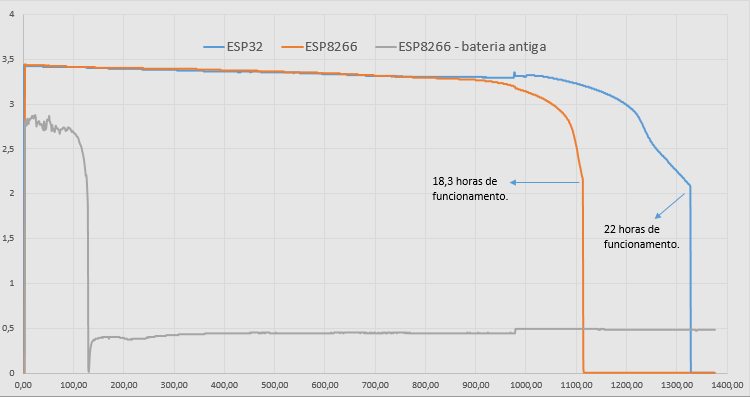
\includegraphics[scale = 0.8]{Graficos/grafico_01.png}
    \caption{Gráfico 1 - Teste sem troca de funções}
    \label{fig:grafico_results_01}
\end{figure}

{
Com base na análise do gráfico 2 de consumo – figura \ref{fig:grafico_results_02}, percebe-se a presença de várias variações bruscas de tensão, esse fato se deve ao modo de funcionamento em que as placas ESPs foram pré-programadas, pois com a troca do modo de operação, ocorre a troca de intensidade do consumo de corrente elétrica. 
}

\begin{figure}[htp]
    \centering
    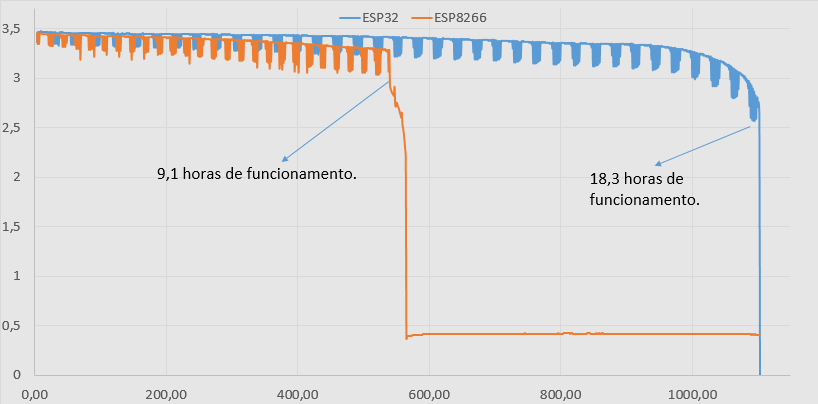
\includegraphics[scale = 0.7]{Graficos/grafico_02.png}
    \caption{Gráfico 2 - Comparativo entre ESP8266 e ESP32}
    \label{fig:grafico_results_02}
\end{figure}

{
Isso é provado a partir da comparação entre o gráfico 1 de consumo – figura \ref{fig:grafico_results_01}, no qual os ESPs não estão programados para realizar a troca de rotina de operações. Desse modo permanecem constantes sem alterar o modo de funcionamento. Por esse motivo não é perceptível nenhuma mudança abrupta no gráfico.
}

{
Devido a tal fato, a vida útil da bateria é fortemente danificada, pois não são preparadas para sofrerem esse tipo de variação de corrente elétrica, sendo percebível em todos os demais testes.
}

\begin{figure}[htp]
    \centering
    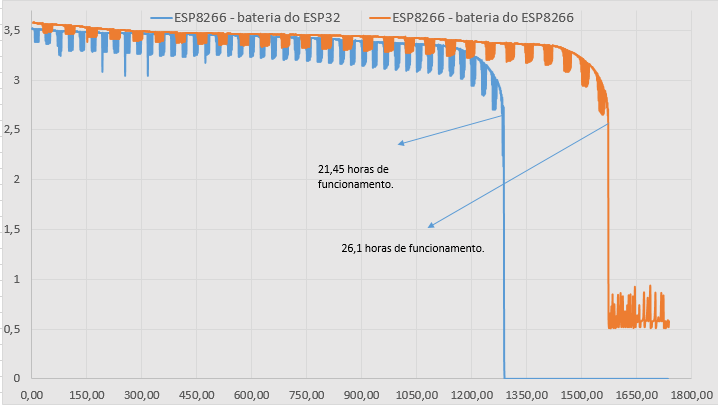
\includegraphics[scale = 0.8]{Graficos/grafico_03.png}
    \caption{Gráfico 3 - Segundo comparativo, mas com as baterias trocadas}
    \label{fig:grafico_results_03}
\end{figure}

\begin{figure}[htp]
    \centering
    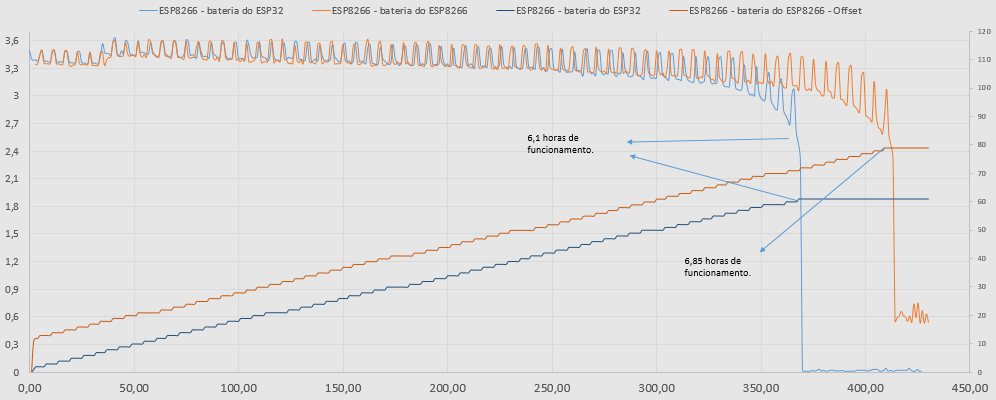
\includegraphics[scale = 0.6]{Graficos/grafico_04.png}
    \caption{Gráfico 4 - Comparativo com contador de ciclos}
    \label{fig:grafico_results_04}
\end{figure}

\begin{figure}[htp]
    \centering
    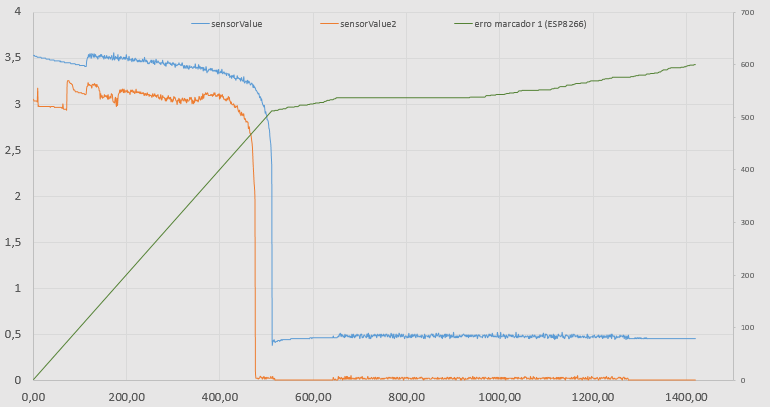
\includegraphics[scale = 0.7]{Graficos/grafico_05.png}
    \caption{Gráfico 5 - Ciclo sem Deep-Sleep ativo.}
    \label{fig:grafico_results_05}
\end{figure}

\begin{figure}[htp]
    \centering
    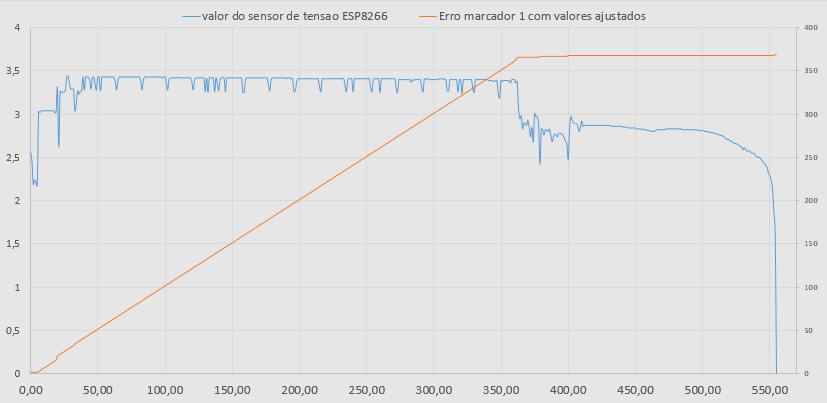
\includegraphics[scale = 0.7]{Graficos/grafico_06.png}
    \caption{Gráfico 6 - Análise de limiar de tensão para funcionamento da placa ESP8266}
    \label{fig:grafico_results_06}
\end{figure}


\newpage
\section{Discussão}
\label{sc:discussao_}


{
A partir dos resultados previamente encontrados, é visto que a característica autonomia e fortemente atingida pelas características de comportamento dos chips ESPs, dessa forma, faz-se necessário o estudo de soluções alternativas para eventualmente corrigir o problema e contornar a baixa vida útil da bateria.
}

{
Em primeiro momento, está sendo visado a utilização do Microcontrolador ATtiny13, como operador central dos comandos, em substituição do ESP, pelo fato de não consumir grandes valores de corrente elétrica. Como transmissor de sinais, está sendo utilizado o módulo NRF24L01, pelos mesmos motivos anunciados ao ATtiny.
}

{
Com essas novas tecnologias, é prevista uma forma de recuperar os altos valores de autonomia demonstrados nos resultados dos testes teóricos, visto que seu comportamento será mais semelhante aos teóricos do que propriamente os dos ESPs.
}


\newpage
\section{Perspectivas de continuidade do trabalho}
\label{sc:continuidade_}

{
Devido aos resultados obtidos, as pesquisas continuarão, todavia, deslocadas para novos microcontroladores, tais como o ATtiny, afim de se obter uma autonomia significativa.
}

{
Para futuras implementações, pode-se estudar a adição de um LDR – Light Dependent Resistor, cuja tradução direta se refere a um resistor dependente de luz. Este componente detecta o início da noite através da variação do seu valor de resistência, e desliga todo o chip até o amanhecer, pois espera-se que o monitoramento não seja de muita significância durante a noite. Podem-se utilizar de outros sensores ou métodos para a detecção do início da noite, mas deve-se atentar ao consumo energético, com a intenção de que este não exceda grandes valores.
}

{
Além disso, pode-se avaliar a possibilidade da utilização de um painel solar integrado ao circuito, com a finalidade de realimentar a bateria e garantir maior autonomia ao projeto. Deve-se salientar que, para que o método funcione, é preciso realizar adaptações nos chips, com a finalidade de torna-los compatíveis com recarga de energia.
}

\newpage
\section{Apêndice A - Tabela de valores de consumo completa}
\label{sc:apendice_a_}

{
Os valores mostrados nessa tabela foram aferidos utilizando 3 multímetros de marcas e modelos diferentes, com a principal finalidade de se chegar a uma média precisa do valor de consumo em cada situação descrita na tabela.
}

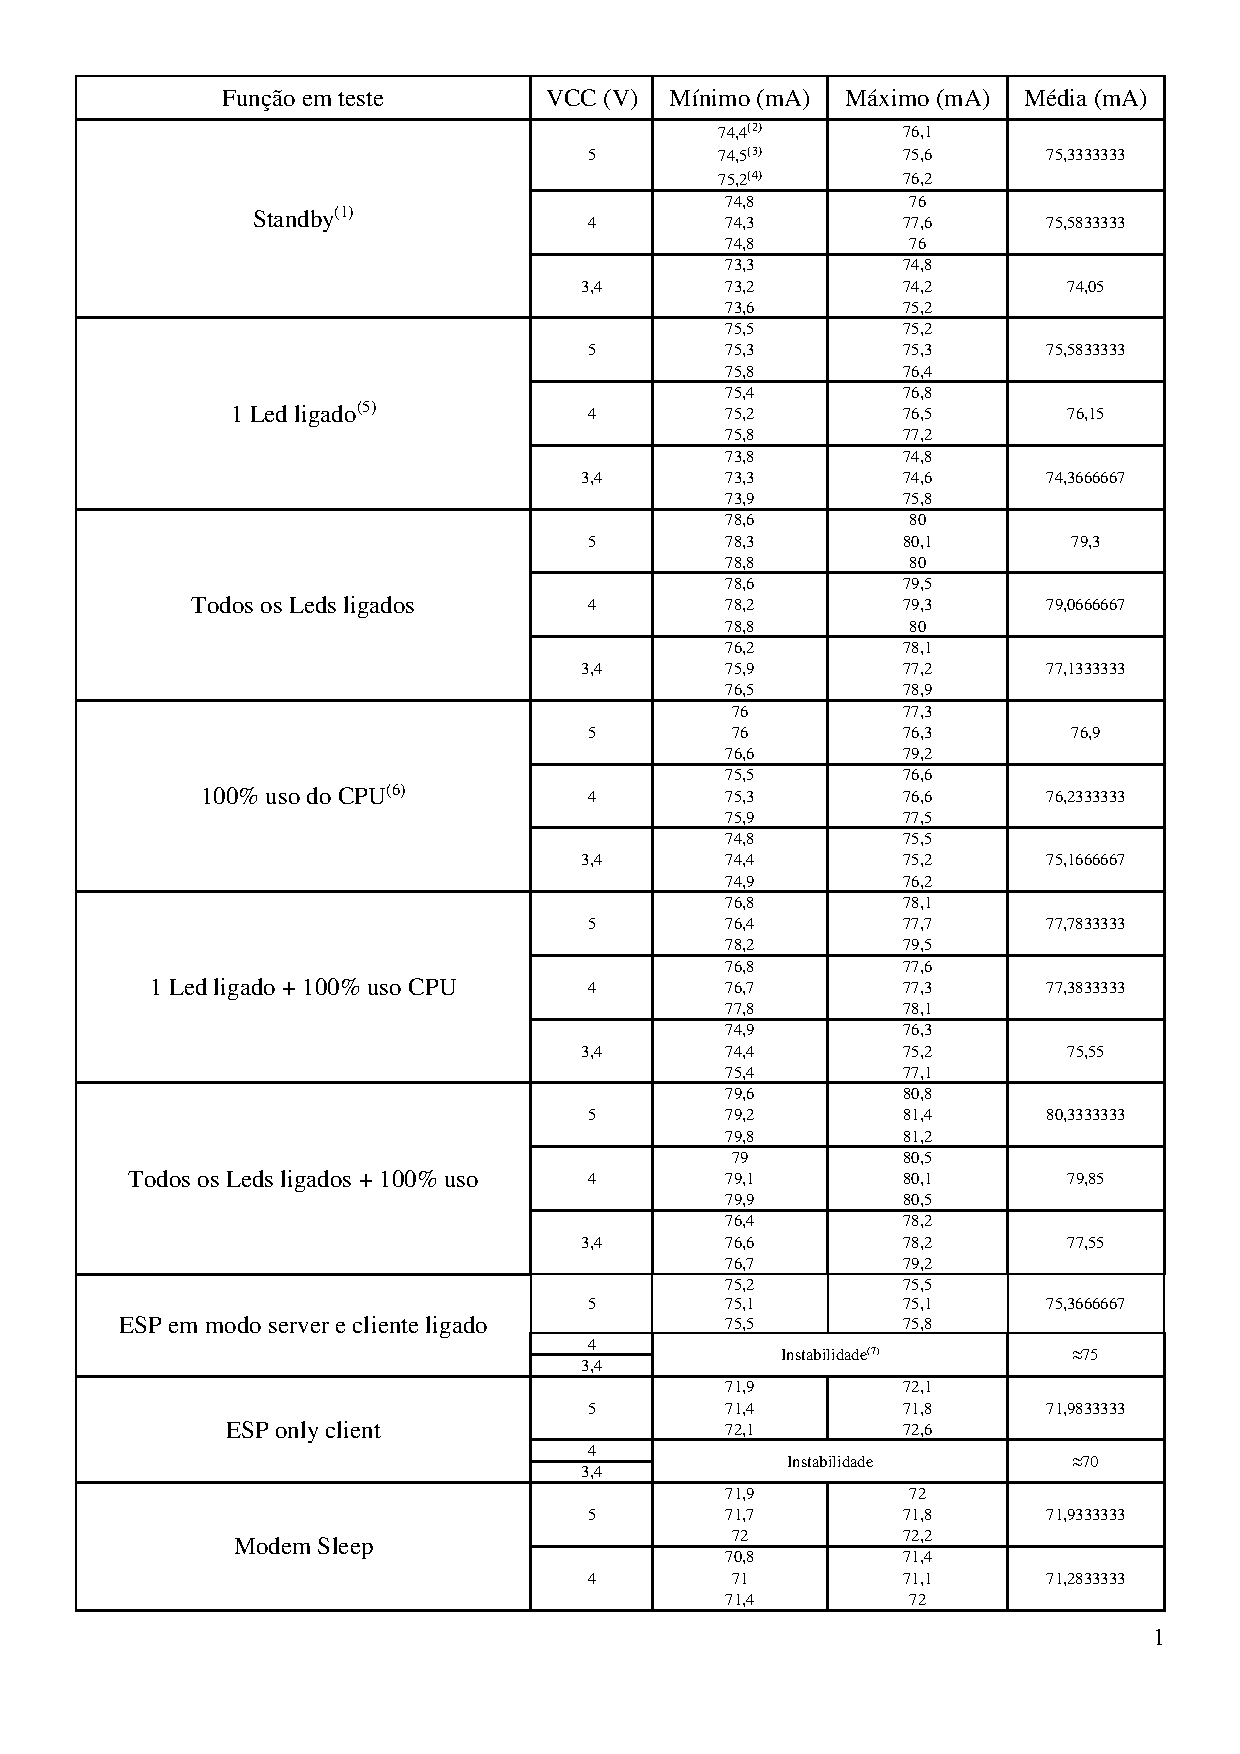
\includepdf[pages=-]{Adicionais/Tabela_valores_de_consumo_ESP.pdf}

\newpage
\section{Apêndice B - Código Modos de Transmissão}
\label{sc:apendice_b_}

\begin{lstlisting}

/*
 * Instituto Federal de Educação, Ciência e Tecnologia Minas Gerais
 * IFMG - Campus Avançado Conselheiro Lafaiete 
 * 
 *  Internet das Vacas código 4
 *  Autor: Jonas Henrique Nascimento
 *  PIBIC-Junior
 * 
 *  Data de início: 11/06/2018
 *  Data da ultima atualização: 22/07/2018
 *  Data de término: 17/06/2018
 *  
 *  Tem o objetivo de estabelecer modelos de transmissão de dados via WiFi.
 *  Cada modelo foi alterado separadamente, sendo necessário o re-upload do
 *  código ao ESP. Cada modo possui vantagens e desvantagens, sendo essas 
 *  incorporadas em sua velocidade de transmissão, potência de alcance ou
 *  consumo de energia.
 *  O código tem a especial necessidade de aferição do consumo energético 
 *  para a futura comparação entre eles. Sendo assim, não foi preocupado 
 *  os dados que seriam transmitidos. A distância entre os nós de toda a 
 *  rede permaneceram constantes durante todos os experimentos.
 *  
 *  Inicialmente, foram testados o modo 802.11b, e seus respectivos valores
 *  de potência de sinal.
 *  Após, testado o 802.11g, e novamente, com seus respectivos valores de 
 *  potência, +20.5 dBm, +18.5 dBm, + 16 dBm e +14 dBm.
 *  Por fim, foi testado o modelo 802.11n. Também com os mesmos valores de
 *  potência de saída.
 * 
 *  Este código está disponível sempre no endereço abaixo, para livre aperfeiçoamento. 
 *  Todavia, pede-se por educação, que ao compartilharem o código, mantenham os autores
 *  originais, tão bem quanto o nome da instituição.
 *  
 *  https://github.com/W8jonas/Internet-das-Vacas/blob/master/programacao/codigo_modos_transmissao/codigo_modos_transmissao.ino
 *  
*/


#include <ESP8266WiFi.h>
#include <WiFiClient.h>
#include <ESP8266WebServer.h>
#include <ESP8266mDNS.h>

extern "C" {
  #include "user_interface.h"
}

const char* ssid = "esp8266";
const char* password = "1234567890";

ESP8266WebServer server(80);

void handleRoot() {

  String textoHTML;

  textoHTML = "Ola!! Aqui &eacute; o <b>ESP8266</b> falando! ";
  textoHTML += "Porta A0: ";
  textoHTML += analogRead(A0);
   
  server.send(200, "text/html", textoHTML);
}

void handleNotFound(){
  String message = "File Not Found\n\n";
  message += "URI: ";
  message += server.uri();
  message += "\nMethod: ";
  message += (server.method() == HTTP_GET)?"GET":"POST";
  message += "\nArguments: ";
  message += server.args();
  message += "\n";
  for (uint8_t i=0; i<server.args(); i++){
    message += " " + server.argName(i) + ": " + server.arg(i) + "\n";
  }
  server.send(404, "text/plain", message);
}

void setup(void){
  Serial.begin(115200);
  
  WiFi.setPhyMode(WIFI_PHY_MODE_11N);
  WiFi.setOutputPower(14);
  WiFi.mode(WIFI_STA);
  WiFi.begin(ssid, password);

//wifi_set_user_fixed_rate;
//wifi_set_user_sup_rate;
//wifi_set_user_rate_limit;

   wifi_set_user_fixed_rate(1, 54);

  Serial.println("");
  int contador = 0;
  while (WiFi.status() != WL_CONNECTED) {
    contador ++;
    delay(50);
    Serial.print("tentativa numero: ");
    Serial.println(contador);
  }
  Serial.println("");
  Serial.print("Conectando em: ");
  Serial.println(ssid);
  Serial.print("IP: ");
  Serial.println(WiFi.localIP());

  server.on("/", handleRoot);

  server.on("/inline", [](){
    server.send(200, "text/plain", "this works as well");
  });

  server.onNotFound(handleNotFound);

  server.begin();
  Serial.println("Servidor iniciado");
}

void loop(void){
  server.handleClient();
}


\end{lstlisting}
\newpage
\section{Apêndice C - Código Modos Wi-Fi}
\label{sc:apendice_c_}


\begin{lstlisting}

/*
 * Instituto Federal de Educação, Ciência e Tecnologia Minas Gerais
 * IFMG - Campus Avançado Conselheiro Lafaiete 
 * 
 *  Internet das Vacas código 3
 *  Autor: Jonas Henrique Nascimento
 *  PIBIC-Junior
 * 
 *  Data de início: 05/06/2018
 *  Data da ultima atualização: 13/08/2018
 *  Data de término: 10/06/2018
 *  
 *  Tem o objetivo de estabelecer modelos de operação de economia de energia.
 *  Sendo, no total, 6 funções. A primeira, abilita o ESP em modo standby, a 
 *  qual nao realiza nenhuma função. Já a segunda, abilita o ESP a trabalhar
 *  em modo client e server ao mesmo tempo. De modo semelhante, a função 3
 *  abilita o ESP a trabalhar somente em modo client. A partir da modo_light_sleep
 *  o ESP recebe sua configuração voltada realmente a economia de energia. 
 *  Sendo o primeiro modelo, o light sleep com a cpu ainda ativa para ser 
 *  inicializada rapidamente. Em contrapartida a próxima função realiza
 *  o light sleep, todavia com a dpu desativada, sendo a unica maneira de
 *  retornar ao estado de funcionamento do ESP por uma interrupção externa.
 *  Por fim, o modelo mais economico, o Deep sleep, a qual deixa o ESP quase
 *  que inteiramente desligado por um período de tempo definido pelo programador.
 *  Toda via, esse modelo requer uma pequena modificação na placa, a qual deverá
 *  constar um jump que interlique a GPIO D0 ao pino Reset do ESP.
 * 
 *  Este código está disponível sempre no endereço abaixo, para livre aperfeiçoamento. 
 *  Todavia, pede-se por educação, que ao compartilharem o código, mantenham os autores
 *  originais, tão bem quanto o nome da instituição.
 *  
 *  https://github.com/W8jonas/Internet-das-Vacas/blob/master/programacao/codigo_modos_wifi/codigo_modos_wifi.ino
 *  
 */

#include <ESP8266WiFi.h>

extern "C" {
  #include "user_interface.h"
}

#define entrada_botao D6

void modo_standby();
void modo_server_and_client();
void modo_only_client();
void modo_modem_sleep();
void modo_light_sleep();
void modo_light_sleep_CPU_OFF();
void modo_DEEP_SLEEP();

int operacao = 0;
boolean leitura = true;

void setup() {
   pinMode(LED_BUILTIN, OUTPUT); 
   pinMode (entrada_botao, INPUT);
   Serial.begin(115200);
}

void loop() {
  leitura = digitalRead(entrada_botao);
  Serial.println(leitura);
  if (leitura == LOW ){
     operacao++;
     delay(500);
  }
   switch (operacao){
      case 0: 
         modo_standby(); 
         break;  // ESP em modo standby
      case 1: 
         modo_server_and_client(); 
         break;  // ESP em modo server and client
      case 2: 
         modo_only_client(); 
         break;  // Esp em modo only client
      case 3: 
         modo_modem_sleep(); 
         break;  // Esp em modem sleep
      case 4: 
         modo_light_sleep(); 
         break;  // Esp em modo light - sleep com cpu ativa
      case 5: 
         modo_light_sleep_CPU_OFF(); 
         break;  // Esp em light - sleep cpu desligada OBS: Para que se possa chegar no deep sleep é preciso comentar a chamada da modo_light_sleep_CPU_OFF.
      case 6:
         modo_DEEP_SLEEP();
         break;  // Esp em deep sleep
      case 7:
      default:
         operacao=0; 
         break;  // 
   }
}

void modo_standby (){
   Serial.println("ESP em modo standby");
}

void modo_server_and_client() {
   Serial.println("ESP em modo server and client");
   WiFi.mode(WIFI_AP);
}

void modo_only_client() {
   Serial.println("Esp em modo only client");
   WiFi.mode(WIFI_STA);
}

void modo_modem_sleep() {
   Serial.println("Esp em modem sleep");
   WiFi.mode(WIFI_OFF);
}

void modo_light_sleep() {
   Serial.println("Esp em modo forçado de sleep");
   wifi_fpm_open();
   WiFi.forceSleepBegin();
   delay(3000);
   WiFi.forceSleepWake();
   wifi_fpm_close();
   wifi_fpm_do_wakeup();
   digitalWrite(LED_BUILTIN, HIGH); delay(200); digitalWrite(LED_BUILTIN, LOW); delay(200);
   digitalWrite(LED_BUILTIN, HIGH); delay(200); digitalWrite(LED_BUILTIN, LOW); delay(200);
}

void modo_light_sleep_CPU_OFF() {
   Serial.println("Esp em modo Light - sleep");
   wifi_station_disconnect();
   wifi_set_opmode(NULL_MODE);
   wifi_fpm_set_sleep_type(LIGHT_SLEEP_T); 
   wifi_fpm_open();
   gpio_pin_wakeup_enable(GPIO_ID_PIN(15), GPIO_PIN_INTR_HILEVEL); 
   Serial.flush();
   wifi_fpm_do_sleep(0xFFFFFFF);
   delay(100);
}

void modo_DEEP_SLEEP() {
   Serial.println("Esp em deep sleep");
   ESP.deepSleep(10000000 , WAKE_RF_DEFAULT);
   delay(100);
}


\end{lstlisting}

\newpage
\section{Apêndice D - Código servidor para teste de consumo}
\label{sc:apendice_d_}

\begin{lstlisting}

/*
 * Instituto Federal de Educação, Ciência e Tecnologia Minas Gerais
 * IFMG - Campus Avançado Conselheiro Lafaiete 
 * 
 *  Internet das Vacas código 3
 *  Autor: Jonas Henrique Nascimento
 *  PIBIC-Junior
 * 
 *  Data de início: 05/06/2018
 *  Data da ultima atualização: 13/08/2018
 *  Data de término: 10/06/2018
 *  
 *  Tem o objetivo de estabelecer modelos de operação de economia de energia.
 *  Sendo, no total, 6 funções. A primeira, abilita o ESP em modo standby, a 
 *  qual nao realiza nenhuma função. Já a segunda, abilita o ESP a trabalhar
 *  em modo client e server ao mesmo tempo. De modo semelhante, a função 3
 *  abilita o ESP a trabalhar somente em modo client. A partir da modo_light_sleep
 *  o ESP recebe sua configuração voltada realmente a economia de energia. 
 *  Sendo o primeiro modelo, o light sleep com a cpu ainda ativa para ser 
 *  inicializada rapidamente. Em contrapartida a próxima função realiza
 *  o light sleep, todavia com a dpu desativada, sendo a unica maneira de
 *  retornar ao estado de funcionamento do ESP por uma interrupção externa.
 *  Por fim, o modelo mais economico, o Deep sleep, a qual deixa o ESP quase
 *  que inteiramente desligado por um período de tempo definido pelo programador.
 *  Toda via, esse modelo requer uma pequena modificação na placa, a qual deverá
 *  constar um jump que interlique a GPIO D0 ao pino Reset do ESP.
 * 
 *  Este código está disponível sempre no endereço abaixo, para livre aperfeiçoamento. 
 *  Todavia, pede-se por educação, que ao compartilharem o código, mantenham os autores
 *  originais, tão bem quanto o nome da instituição.
 *  
 *  https://github.com/W8jonas/Internet-das-Vacas/blob/master/programacao/codigo_modos_wifi/codigo_modos_wifi.ino
 *  
 */

#include <ESP8266WiFi.h>

extern "C" {
  #include "user_interface.h"
}

#define entrada_botao D6

void modo_standby();
void modo_server_and_client();
void modo_only_client();
void modo_modem_sleep();
void modo_light_sleep();
void modo_light_sleep_CPU_OFF();
void modo_DEEP_SLEEP();

int operacao = 0;
boolean leitura = true;

void setup() {
   pinMode(LED_BUILTIN, OUTPUT); 
   pinMode (entrada_botao, INPUT);
   Serial.begin(115200);
}

void loop() {
  leitura = digitalRead(entrada_botao);
  Serial.println(leitura);
  if (leitura == LOW ){
     operacao++;
     delay(500);
  }
   switch (operacao){
      case 0: 
         modo_standby(); 
         break;  // ESP em modo standby
      case 1: 
         modo_server_and_client(); 
         break;  // ESP em modo server and client
      case 2: 
         modo_only_client(); 
         break;  // Esp em modo only client
      case 3: 
         modo_modem_sleep(); 
         break;  // Esp em modem sleep
      case 4: 
         modo_light_sleep(); 
         break;  // Esp em modo light - sleep com cpu ativa
      case 5: 
         modo_light_sleep_CPU_OFF(); 
         break;  // Esp em light - sleep cpu desligada OBS: Para que se possa chegar no deep sleep é preciso comentar a chamada da modo_light_sleep_CPU_OFF.
      case 6:
         modo_DEEP_SLEEP();
         break;  // Esp em deep sleep
      case 7:
      default:
         operacao=0; 
         break;  // 
   }
}

void modo_standby (){
   Serial.println("ESP em modo standby");
}

void modo_server_and_client() {
   Serial.println("ESP em modo server and client");
   WiFi.mode(WIFI_AP);
}

void modo_only_client() {
   Serial.println("Esp em modo only client");
   WiFi.mode(WIFI_STA);
}

void modo_modem_sleep() {
   Serial.println("Esp em modem sleep");
   WiFi.mode(WIFI_OFF);
}

void modo_light_sleep() {
   Serial.println("Esp em modo forçado de sleep");
   wifi_fpm_open();
   WiFi.forceSleepBegin();
   delay(3000);
   WiFi.forceSleepWake();
   wifi_fpm_close();
   wifi_fpm_do_wakeup();
   digitalWrite(LED_BUILTIN, HIGH); delay(200); digitalWrite(LED_BUILTIN, LOW); delay(200);
   digitalWrite(LED_BUILTIN, HIGH); delay(200); digitalWrite(LED_BUILTIN, LOW); delay(200);
}

void modo_light_sleep_CPU_OFF() {
   Serial.println("Esp em modo Light - sleep");
   wifi_station_disconnect();
   wifi_set_opmode(NULL_MODE);
   wifi_fpm_set_sleep_type(LIGHT_SLEEP_T); 
   wifi_fpm_open();
   gpio_pin_wakeup_enable(GPIO_ID_PIN(15), GPIO_PIN_INTR_HILEVEL); 
   Serial.flush();
   wifi_fpm_do_sleep(0xFFFFFFF);
   delay(100);
}

void modo_DEEP_SLEEP() {
   Serial.println("Esp em deep sleep");
   ESP.deepSleep(10000000 , WAKE_RF_DEFAULT);
   delay(100);
}


\end{lstlisting}
\newpage
\section{Apêndice E - Código testes de consumo}
\label{sc:apendice_e_}

\begin{lstlisting}

/*
 * Instituto Federal de Educação, Ciência e Tecnologia Minas Gerais
 * IFMG - Campus Avançado Conselheiro Lafaiete 
 * 
 *  Internet das Vacas código 3
 *  Autor: Jonas Henrique Nascimento
 *  PIBIC-Junior
 * 
 *  Data de início: 13/08/2018
 *  Data da ultima atualização: 15/09/2018
 *  Data de término: 02/09/2018
 *  
 *  Tem o objetivo de estabelecer modelos de operação de economia de energia.
 *  Sendo, no total, 6 funções. A primeira, abilita o ESP em modo standby, a 
 *  qual nao realiza nenhuma função. Já a segunda, abilita o ESP a trabalhar
 *  em modo client e server ao mesmo tempo. De modo semelhante, a função 3
 *  abilita o ESP a trabalhar somente em modo client. A partir da modo_light_sleep
 *  o ESP recebe sua configuração voltada realmente a economia de energia. 
 *  Sendo o primeiro modelo, o light sleep com a cpu ainda ativa para ser 
 *  inicializada rapidamente. Em contrapartida a próxima função realiza
 *  o light sleep, todavia com a dpu desativada, sendo a unica maneira de
 *  retornar ao estado de funcionamento do ESP por uma interrupção externa.
 *  Por fim, o modelo mais economico, o Deep sleep, a qual deixa o ESP quase
 *  que inteiramente desligado por um período de tempo definido pelo programador.
 *  Toda via, esse modelo requer uma pequena modificação na placa, a qual deverá
 *  constar um jump que interlique a GPIO D0 ao pino Reset do ESP.
 * 
 *  Este código está disponível sempre no endereço abaixo, para livre aperfeiçoamento. 
 *  Todavia, pede-se por educação, que ao compartilharem o código, mantenham os autores
 *  originais, tão bem quanto o nome da instituição.
 *  
 *  https://github.com/W8jonas/Internet-das-Vacas/blob/master/programacao/codigo_teste_de_consumo/codigo_teste_de_consumo.ino
 *  
 */


#include <ESP8266WiFi.h>
#include <WiFiClient.h>
#include <ESP8266WebServer.h>
#include <ESP8266mDNS.h>

#define tempo_para_desligar 250000
#define tempo_modo_funcionamento 200000
#define tempo_modo_funcionamento2 250000

#define Pino_transmit D8

extern "C" {
  #include "user_interface.h"
}

void modo_DEEP_SLEEP();
void handleNotFound();
void handleRoot();
void MAX_CPU();

const char* ssid = "82W8JH";
const char* password = "w8989jonas";

ESP8266WebServer server(80);

void setup() {
  
   Serial.begin(115200);
   Serial.println("Inicializando o setup");
   WiFi.setPhyMode(WIFI_PHY_MODE_11N);
   WiFi.setOutputPower(14);
   WiFi.mode(WIFI_STA);
   WiFi.begin(ssid, password);
   wifi_set_user_fixed_rate(1, 54);
   int contador = 0;

   pinMode(Pino_transmit, OUTPUT);
   digitalWrite(Pino_transmit, HIGH);
   
   while (WiFi.status() != WL_CONNECTED) {
      contador ++;
      delay(50);
   }

   server.on("/", handleRoot);
   server.on("/inline", [] () { server.send(200, "text/plain", "this works as well"); } );

   server.onNotFound(handleNotFound);
   server.begin();
   delay(500);
   
   Serial.println("");
   Serial.print("Conectando em: ");
   Serial.println(ssid);
   Serial.print("IP: ");
   Serial.println(WiFi.localIP());
}


void loop() {
   unsigned long valor_atual_contador = millis();
   Serial.println(valor_atual_contador);
   digitalWrite(Pino_transmit, LOW);
   if (valor_atual_contador < tempo_modo_funcionamento) {
      MAX_CPU();
      digitalWrite(Pino_transmit, LOW);
   }
   
   if ((valor_atual_contador >= tempo_modo_funcionamento) && (valor_atual_contador < tempo_modo_funcionamento2)) {
      server.handleClient();
      handleRoot();
   }
   
   if (valor_atual_contador >= tempo_para_desligar) {
      modo_DEEP_SLEEP();
   }
   
}


void MAX_CPU() {
   Serial.println("MAX_CPU");
   int cont = 1;
   float resp = 1;
   float resp2 = 1;
   for(int AA = 0; AA < 500; AA++){
      resp = 3 + sin(resp)/cos(resp*resp/2) * sqrt(sqrt(resp*resp));
      resp = resp * 0.5;
      resp2 = sqrt(AA);
      yield();
  }
}


void handleRoot() {
   Serial.println("HandleRoot");
   String textoHTML;
   textoHTML = " PARA DE ME COPIAR DANIELLE ";
   server.send(200, "text/html", textoHTML);
}


void handleNotFound(){
   Serial.println("handleNotFound");
   String message = "Sem arquivo\n\n";
   message += "URI: ";
   message += server.uri();
   message += "\nMethod: ";
   message += (server.method() == HTTP_GET)?"GET":"POST";
   message += "\nArguments: ";
   message += server.args();
   message += "\n";
   for (uint8_t i=0; i<server.args(); i++){
     message += " " + server.argName(i) + ": " + server.arg(i) + "\n";
   }
   server.send(404, "text/plain", message);
}


void modo_DEEP_SLEEP() {
   digitalWrite(Pino_transmit, LOW);
   digitalWrite(Pino_transmit, HIGH);
   delay(800);
   digitalWrite(Pino_transmit, LOW);
   Serial.println("Deep-Sleep");
   delay(500);
   ESP.deepSleep(100000000 , WAKE_RF_DEFAULT);
   delay(500);
}


\end{lstlisting}
\newpage
\section{Apêndice F - Código testes de consumo ESP32}
\label{sc:apendice_f_}


\begin{lstlisting}

/*
 * Instituto Federal de Educação, Ciência e Tecnologia Minas Gerais
 * IFMG - Campus Avançado Conselheiro Lafaiete 
 * 
 *  Internet das Vacas código 3
 *  Autor: Jonas Henrique Nascimento
 *  PIBIC-Junior
 * 
 *  Data de início: 13/08/2018
 *  Data da ultima atualização: 02/09/2018
 *  Data de término: 02/09/2018
 *  
 *  Tem o objetivo de estabelecer modelos de operação de economia de energia.
 *  Sendo, no total, 6 funções. A primeira, abilita o ESP em modo standby, a 
 *  qual nao realiza nenhuma função. Já a segunda, abilita o ESP a trabalhar
 *  em modo client e server ao mesmo tempo. De modo semelhante, a função 3
 *  abilita o ESP a trabalhar somente em modo client. A partir da modo_light_sleep
 *  o ESP recebe sua configuração voltada realmente a economia de energia. 
 *  Sendo o primeiro modelo, o light sleep com a cpu ainda ativa para ser 
 *  inicializada rapidamente. Em contrapartida a próxima função realiza
 *  o light sleep, todavia com a dpu desativada, sendo a unica maneira de
 *  retornar ao estado de funcionamento do ESP por uma interrupção externa.
 *  Por fim, o modelo mais economico, o Deep sleep, a qual deixa o ESP quase
 *  que inteiramente desligado por um período de tempo definido pelo programador.
 *  Toda via, esse modelo requer uma pequena modificação na placa, a qual deverá
 *  constar um jump que interlique a GPIO D0 ao pino Reset do ESP.
 * 
 *  Este código está disponível sempre no endereço abaixo, para livre aperfeiçoamento. 
 *  Todavia, pede-se por educação, que ao compartilharem o código, mantenham os autores
 *  originais, tão bem quanto o nome da instituição.
 *  
 *  https://github.com/W8jonas/Internet-das-Vacas/blob/master/programacao/codigo_teste_de_consumo_ESP32/codigo_teste_de_consumo_ESP32.ino
 *  
*/


#include <WiFi.h>

#define tempo_para_desligar 25000
#define tempo_modo_funcionamento 20000
#define tempo_modo_funcionamento2 25000
#define Pino_transmit 4

void modo_DEEP_SLEEP();
void Servidor_ON(unsigned long contador_interno);
void MAX_CPU();

const char* ssid = "82W8JH";
const char* password = "w8989jonas";

WiFiServer server(80);



void setup() {
  
   Serial.begin(115200);
   Serial.println("Inicializando o setup");
   
 //  WiFi.setPhyMode(WIFI_PHY_MODE_11N);
 //  WiFi.setOutputPower(14);
 //  WiFi.mode(WIFI_STA);
   
   WiFi.begin(ssid, password);
 //  wifi_set_user_fixed_rate(1, 54);
   
   int contador = 0;
   
   while (WiFi.status() != WL_CONNECTED) {
      contador ++;
      delay(50);
   }

   server.begin();
   delay(500);
   
   Serial.println("");
   Serial.print("Conectando em: ");
   Serial.println(ssid);
   Serial.print("IP: ");
   Serial.println(WiFi.localIP());
   esp_sleep_enable_timer_wakeup(100000000);

   pinMode(Pino_transmit, OUTPUT);
   digitalWrite(Pino_transmit, HIGH);
}


void loop() {
   unsigned long valor_atual_contador = millis();
   Serial.println(valor_atual_contador);
   
   if (valor_atual_contador < tempo_modo_funcionamento) {
      MAX_CPU();
   } 
   
   if ((valor_atual_contador >= tempo_modo_funcionamento) && (valor_atual_contador < tempo_modo_funcionamento2)) {
      Servidor_ON(valor_atual_contador);
   }
   
//   client.stop();
   
   if (valor_atual_contador >= tempo_para_desligar) {
      modo_DEEP_SLEEP();
   }
   
}


void MAX_CPU() {
   Serial.println("MAX_CPU");
   int cont = 1;
   float resp = 1;
   float resp2 = 1;
   for(int AA = 0; AA < 500; AA++){
      resp = 3 + sin(resp)/cos(resp*resp/2) * sqrt(sqrt(resp*resp));
      resp = resp * 0.5;
      resp2 = sqrt(AA);
      yield();
  }
}

void Servidor_ON(unsigned long valor_cont){
    
    WiFiClient client = server.available();
    String currentLine = "";                // make a String to hold incoming data from the client
    while (client.connected()) {            // loop while the client's connected
      if (client.available()) {             // if there's bytes to read from the client,
        char c = client.read();             // read a byte, then
        Serial.write(c);                    // print it out the serial monitor
        if (c == '\n') {                    // if the byte is a newline character

          // if the current line is blank, you got two newline characters in a row.
          // that's the end of the client HTTP request, so send a response:
          if (currentLine.length() == 0) {
            // HTTP headers always start with a response code (e.g. HTTP/1.1 200 OK)
            // and a content-type so the client knows what's coming, then a blank line:
            client.println("HTTP/1.1 200 OK");
            client.println("Content-type:text/html");
            client.println();

            // the content of the HTTP response follows the header:
            client.print("Contador");
            client.print(valor_cont);

            // The HTTP response ends with another blank line:
            client.println();
            // break out of the while loop:
            break;
          } else {    // if you got a newline, then clear currentLine:
            currentLine = "";
          }
        } else if (c != '\r') {  // if you got anything else but a carriage return character,
          currentLine += c;      // add it to the end of the currentLine
        }

      }
    }


}

void modo_DEEP_SLEEP() {
   digitalWrite(Pino_transmit, LOW);
   digitalWrite(Pino_transmit, HIGH);
   delay(800);
   digitalWrite(Pino_transmit, LOW);
  
   Serial.println("Deep-Sleep");
   delay(500);
   esp_deep_sleep_start();
   delay(500);
}


\end{lstlisting}
\newpage
\section{Apêndice G - Código servidor de consumo V2}
\label{sc:apendice_g_}

\begin{lstlisting}

/*
 * Instituto Federal de Educação, Ciência e Tecnologia Minas Gerais
 * IFMG - Campus Avançado Conselheiro Lafaiete 
 * 
 * Internet das Vacas código 2
 * Autor: Jonas Henrique Nascimento
 * PIBIC-Junior
 * 
 * Data de início: 06/04/2018
 * Data da ultima atualização: 13/05/2018
 * Data de término: 13/05/2018
 * 
 * Tem o objetivo de estabelecer um servidor dentro do ESP que possibilite ligar 8 LEDs independentes e optar por 2 estados de processamento;
 * O primeiro, a qual não será realizado nenhuma operação adicional além do próprio servidor.
 * No segundo, o processador, além de manter o próprio servidor, executará contas aritméticas adicinais afim de se usar 100% da CPU.
 * O propósito do programa é a relaziação dos teste com relação ao consumo da placa.
 *
 *  Este código está disponível sempre no endereço abaixo, para livre aperfeiçoamento. 
 *  Todavia, pede-se por educação, que ao compartilharem o código, mantenham os autores
 *  originais, tão bem quanto o nome da instituição.
 *
 * https://github.com/W8jonas/Internet-das-Vacas/blob/master/programacao/codigo_do_servidor---consumov2/codigo_do_servidor---consumov2.ino
 *  
*/


#include <ESP8266WiFi.h>

const char* ssid = "esp8266";
const char* password = "1234567890";

WiFiServer server(80); //Shield irá receber as requisições das páginas (o padrão WEB é a porta 80)

String HTTP_req; 
String URLValue;

void processaPorta(byte porta, byte posicao, WiFiClient cl);
void lePortaDigital(byte porta, byte posicao, WiFiClient cl);
void lePortaAnalogica(byte porta, byte posicao, WiFiClient cl);

void conta_1();
  
String getURLRequest(String *requisicao);
bool mainPageRequest(String *requisicao);

const byte qtdePinosDigitais = 9;
byte pinosDigitais[qtdePinosDigitais] = {2      , 0      , 4      , 5      , 15     , 13     , 12      , 14      , 16     };
byte modoPinos[qtdePinosDigitais]     = {OUTPUT , OUTPUT , OUTPUT , OUTPUT , OUTPUT , OUTPUT , OUTPUT  , OUTPUT  , OUTPUT };
boolean flag = true;
int condicao = 2;



void setup(){
    Serial.begin(115200);

    Serial.println();
    Serial.print("Conectando a ");
    Serial.println(ssid);

    WiFi.begin(ssid, password);

    while (WiFi.status() != WL_CONNECTED) {
      delay(500);
      Serial.print(".");
    }
    Serial.println("");
    Serial.println("WiFi conectado!");


    server.begin();
    Serial.println("Server iniciado");

    Serial.println(WiFi.localIP());
    
    for (int nP=0; nP < qtdePinosDigitais; nP++) {
        pinMode(pinosDigitais[nP], modoPinos[nP]);
    }
}


void loop(){

    WiFiClient  client = server.available();

    if (client) { 
        boolean currentLineIsBlank = true;
        while (client.connected()) {
            if (client.available()) { 
                char c = client.read(); 
                HTTP_req += c;  
                
                if (c == '\n' && currentLineIsBlank ) { 

                    if ( mainPageRequest(&HTTP_req) ) {
                        URLValue = getURLRequest(&HTTP_req);
                        Serial.println(HTTP_req);
                                                 
                        client.println("HTTP/1.1 200 OK");
                        client.println("Content-Type: text/html");
                        client.println("Connection: keep-alive");              
                        client.println();
                        
                        //Conteudo da Página HTML
                        client.println("<!DOCTYPE html>");
                        client.println("<html>");

                        client.println("<head>");
                        client.println("<title>Servidor de teste</title>");

                        client.println("<script>");
                        client.println("function LeDadosDoArduino() {");
                        client.println("nocache = \"&nocache=\" + Math.random() * 1000000;");
                        client.println("var request = new XMLHttpRequest();");
                        client.println("var posIni;");
                        client.println("var valPosIni;");
                        client.println("var valPosFim;");
                        client.println("request.onreadystatechange = function() {");
                        client.println("if (this.readyState == 4) {");
                        client.println("if (this.status == 200) {");
                        client.println("if (this.responseText != null) {");

                        for (int nL=0; nL < qtdePinosDigitais; nL++) {                                                 
                            client.print("posIni = this.responseText.indexOf(\"PD");
                            client.print(pinosDigitais[nL]);
                            client.println("\");");
                            client.println("if ( posIni > -1) {");
                            client.println("valPosIni = this.responseText.indexOf(\"#\", posIni) + 1;");
                            client.println("valPosFim = this.responseText.indexOf(\"|\", posIni);");
                            client.print("document.getElementById(\"pino");
                            client.print(pinosDigitais[nL]);
                            client.println("\").checked = Number(this.responseText.substring(valPosIni, valPosFim));");
                            client.println("}");
                        }


                        client.println("}}}}");
                        client.println("request.open(\"GET\", \"solicitacao_via_ajax\" + nocache, true);");
                        client.println("request.send(null);");
                        client.println("setTimeout('LeDadosDoArduino()', 5000);");
                        client.println("}");
                        client.println("</script>");
                        
                        client.println("</head>");

                        client.println("<body onload=\"LeDadosDoArduino()\">");                                     
                        client.println("<h1>Porta analogica</h1>");

                        client.println("<br/>");                        
                        client.println("<h1>PORTAS digitais</h1>");
                        client.println("<form method=\"get\">");

                        for (int nL=0; nL < qtdePinosDigitais; nL++) {
                            processaPorta(pinosDigitais[nL], nL, client);
                            client.println("<br/>");
                        }
                        
                        client.println("<button type=\"submit\">Envia as opcoes para o ESP8266</button>");
                        client.println("</form>");                      
                        
                        client.println("</body>");
                        
                        client.println("</html>");
                    
                    } else if (HTTP_req.indexOf("solicitacao_via_ajax") > -1) {  

                        Serial.println(HTTP_req);

                        client.println("HTTP/1.1 200 OK");
                        client.println("Content-Type: text/html");
                        client.println("Connection: keep-alive");      
                        client.println();                      


                        for (int nL=0; nL < qtdePinosDigitais; nL++) {
                            lePortaDigital(pinosDigitais[nL], nL, client);
                        }
                            
                    } else {

                        Serial.println(HTTP_req);
                        client.println("HTTP/1.1 200 OK");
                    }
                    HTTP_req = "";    
                    break;
                }
                
                if (c == '\n') {
                    currentLineIsBlank = true;
                } 
                else if (c != '\r') {
                    currentLineIsBlank = false;
                }
            }
        } 
        delay(1);     
        client.stop(); 
    } 

  if(condicao == 1)conta_1();
  
}


void processaPorta(byte porta, byte posicao, WiFiClient cl){
static boolean LED_status = 0;
String cHTML;
   
    cHTML = "P";
    cHTML += porta;
    cHTML += "=";
    cHTML += porta;

    if (modoPinos[posicao] == OUTPUT) { 
        
        if (URLValue.indexOf(cHTML) > -1) { 
           LED_status = HIGH;
        } else {
           LED_status = LOW;
        }
        if((porta == 16) && (LED_status == HIGH)){
          condicao = 1;
        } else{
          condicao = 0;
        }
        digitalWrite(porta, LED_status);
    } else {

        LED_status = digitalRead(porta);
    }

    cl.print("<input type=\"checkbox\" name=\"P");
    cl.print(porta);
    cl.print("\" value=\"");
    cl.print(porta);
    
    cl.print("\"");

    cl.print(" id=\"pino");        
    cl.print(porta);
    cl.print("\"");
    
    if (LED_status) { 
        cl.print(" checked ");
    }

    if (modoPinos[posicao] != OUTPUT) { 
        cl.print(" disabled ");
    }
    
    cl.print(">Porta ");
    cl.print(porta);

    cl.println();
}


void lePortaDigital(byte porta, byte posicao, WiFiClient cl){
    if (modoPinos[posicao] != OUTPUT) { 
       cl.print("PD");
       cl.print(porta);
       cl.print("#");
       
       if (digitalRead(porta)) {
          cl.print("1");
       } else {
          cl.print("0");
       }
       cl.println("|");
    }
}


void lePortaAnalogica(byte porta, byte posicao, WiFiClient cl){
   cl.print("PA");
   cl.print(porta);
   cl.print("#");
   
   cl.print(analogRead(porta));

   //especifico para formatar o valor da porta analogica A0
   if (porta == A0) { 
      cl.print(" (");
      cl.print(map(analogRead(A0),0,1023,0,179)); 
      cl.print("&deg;)");
   }
   
   cl.println("|");   
}


String getURLRequest(String *requisicao) {
int inicio, fim;
String retorno;

  inicio = requisicao->indexOf("GET") + 3;
  fim = requisicao->indexOf("HTTP/") - 1;
  retorno = requisicao->substring(inicio, fim);
  retorno.trim();

  return retorno;
}


bool mainPageRequest(String *requisicao) {
  
  
String valor;
bool retorno = false;

  valor = getURLRequest(requisicao);
  valor.toLowerCase();

  if (valor == "/") {
     retorno = true;
  }

  if (valor.substring(0,2) == "/?") {
     retorno = true;
  }  

  if (valor.substring(0,10) == "/index.htm") {
     retorno = true;
  }  

  return retorno;
}


void conta_1(){  
  int cont = 1;
  float resp = 1;
  float resp2 = 1;
  for(int AA = 0; AA < 500; AA++){
     resp = 3 + sin(resp)/cos(resp*resp/2) * sqrt(sqrt(resp*resp));
     resp = resp * 0.5;
     Serial.println(resp);
     Serial.print("   ");
     resp2 = sqrt(AA);
     Serial.print(resp2);
     Serial.print("   ");
     yield();
  }
}

\end{lstlisting}


\newpage


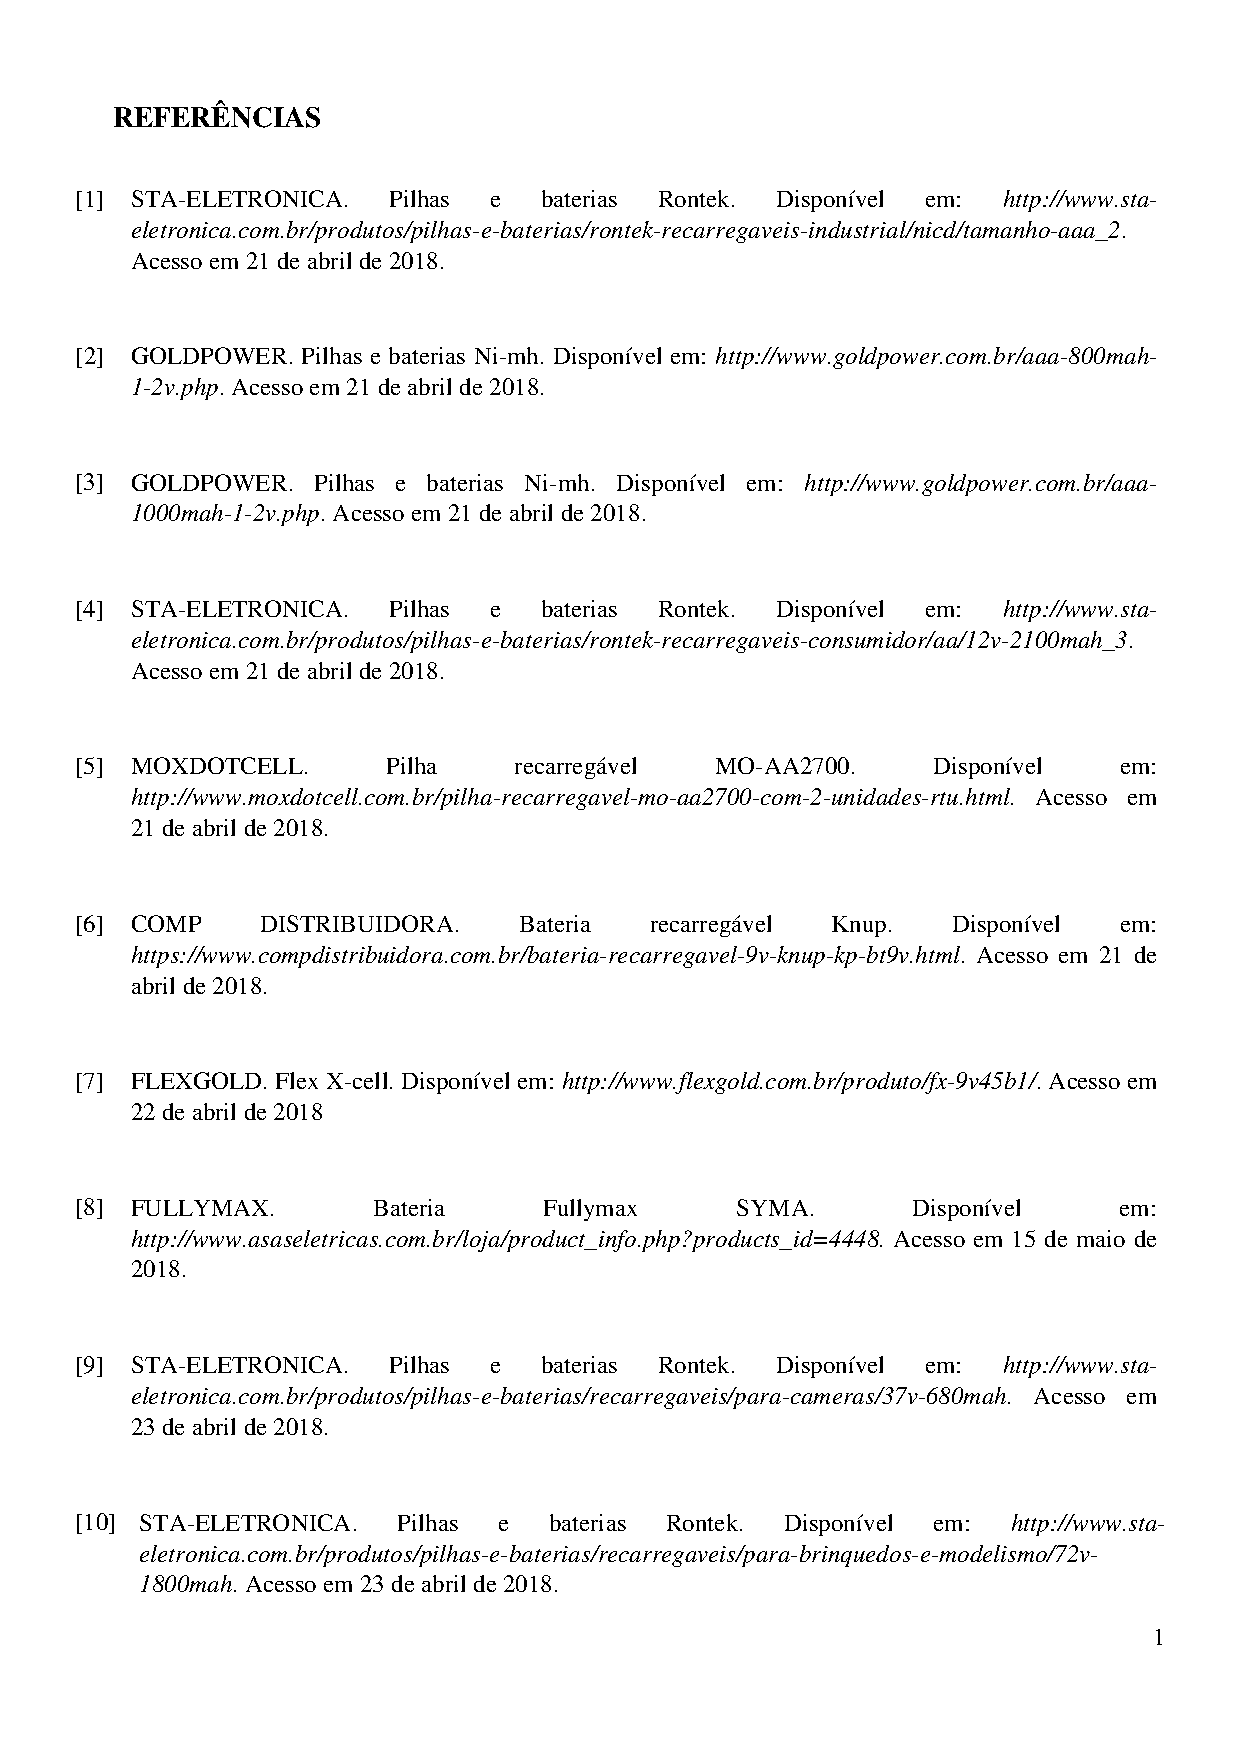
\includepdf[pages=-]{Adicionais/referencias.pdf}

\end{document}